\documentclass{eic-bcc-tcc}

\usepackage{float}
\usepackage{subcaption}

%-----------------------------------------------
% Metadados do Trabalho
%-----------------------------------------------
\title{RageFilter: Construção de um Dataset de Toxicidade para Comunidades \textit{gamer} Brasileiras}
\titleen{RageFilter: Building a Toxicity Dataset for Brazilian Gaming Communities}


% Nome completo do/da(s) autor(es)
% \addstudent[Full Name]{Nome Completo}
% O comando recebe um parâmetro opcional para a formatação dos nomes em inglÊs
\addstudent[Luiz Henrique Mendes de Oliveira Castro]{Luiz Henrique Mendes de Oliveira Castro}

\advisor{lo AMarcerêas Rodrigues da Silva, D.Sc.} 

% Membros da Banca para folha de aprovação
\addboardmember{Membro Interno}{Nome Membro Interno, D.Sc.\footnotemark[1]}
\addboardmember{Membro Externo}{Nome Membro Externo, D.Sc.\footnotemark[1] \footnotetext[1]{Caso a titulação não seja D.Sc., utilizar a adequada (p.ex., Dr. Ing., M.Sc., Esp., entre outras)}}

% Ano da defesa
\date{2026}


%-----------------------------------------------
% Abreviações
%-----------------------------------------------
% \newacronym{label}{sigla}{descrição} - Define um novo acrônimo
\newacronym{cefet}{Cefet/RJ}{Centro Federal de Educação Tecnológica Celso Suckow da Fonseca}
\newacronym{tcc}{TCC}{Trabalho de Conlusão de Curso}
\newacronym{abnt}{ABNT}{Associação Brasileira de Normas Técnicas}
\newacronym{ia}{IA}{Inteligência Artificial}


\begin{document}

%-----------------------------------------------
% Elementos pré-textuais
%-----------------------------------------------
\maketitle

\begin{dedicatoria}
Dedico este TCC aos meus pais e à minha namorada, por todo o amor, apoio e força que me acompanharam nesta caminhada.
\end{dedicatoria}


\begin{agradecimentos}
Agradeço, primeiramente, ao meu professor, cuja orientação, paciência e dedicação foram fundamentais para o desenvolvimento deste Trabalho de Conclusão de Curso. Sua capacidade de ensinar e incentivar o pensamento crítico foram essenciais para que eu pudesse evoluir ao longo desse processo.

Aos meus pais, deixo meu mais profundo agradecimento pelo amor incondicional, apoio constante e pela base sólida que sempre me proporcionaram. Sem eles, esta conquista não seria possível.

À minha namorada, agradeço pela compreensão nos momentos de ausência, pelo incentivo diário e por acreditar em mim mesmo mesmo quando eu duvidava. Sua parceria tornou esta jornada muito mais leve.

Ao meu primo, minha tia e minha avó, sou grato pelo apoio, carinho e pela torcida constante, sempre me lembrando da importância desta etapa.

Aos meus amigos da escola e da faculdade, agradeço pela parceria, pelas conversas, pela troca de conhecimentos e por tornarem o caminho mais divertido e menos solitário. Cada um de vocês contribuiu, de alguma forma, para que eu chegasse até aqui.

A todos que, direta ou indiretamente, fizeram parte desta trajetória, deixo minha sincera gratidão.

Por fim, agradeço ao CEFET/RJ, instituição que me acompanha desde 2021 e que foi fundamental na minha formação acadêmica, oferecendo estrutura, conhecimento e oportunidades que contribuíram profundamente para o meu crescimento pessoal e profissional.
\end{agradecimentos}

\begin{resumo}
O crescimento das comunidades digitais de jogos eletrônicos tem intensificado a ocorrência de interações tóxicas em plataformas digitais associadas a jogos eletrônicos, como a Twitch. Apesar da existência de pesquisas sobre toxicidade textual, ainda há escassez de \textit{datasets} em português voltados especificamente para a linguagem \textit{gamer}, marcada por gírias, abreviações e expressões próprias desse contexto. Este trabalho propõe a construção de um \textit{dataset} de toxicidade direcionado às comunidades \textit{gamer} brasileiras, contendo mensagens rotuladas e uma taxonomia de termos ofensivos utilizada em ambientes de jogos \textit{on-line}. A metodologia envolve a coleta de mensagens em plataformas digitais, o processo de limpeza e padronização textual, a definição de categorias de toxicidade e a elaboração de estratégias de anotação e tokenização das mensagens. Além disso, pretende-se construir um repositório complementar contendo gírias e expressões ofensivas características da comunidade \textit{gamer}. Como contribuição, o trabalho busca disponibilizar um recurso especializado para pesquisas futuras em Processamento de Linguagem Natural e detecção de toxicidade em português brasileiro.
\palavraschave{Toxicidade em jogos. Processamento de Linguagem Natural. \textit{Dataset}. Comunidades \textit{gamer}. Toxicidade textual.}
\end{resumo}


\begin{abstract}
\textit{The growth of digital gaming communities has intensified toxic interactions on digital platforms associated with electronic games, such as Twitch. Although studies on textual toxicity already exist, there is still a lack of Portuguese datasets specifically focused on \textit{gamer} language, which is characterized by slang, abbreviations, and expressions typical of online gaming environments. This work proposes the construction of a toxicity dataset aimed at Brazilian gaming communities, containing labeled messages and a taxonomy of offensive terms used in online games. The methodology involves collecting messages from digital platforms, performing text cleaning and standardization, defining toxicity categories, and developing annotation and tokenization strategies. In addition, a complementary repository containing \textit{gamer} slang and offensive expressions commonly used by players will be created. As a contribution, the work aims to provide a specialized resource for future research in Natural Language Processing and toxicity detection in Brazilian Portuguese.}

\keywords{\textit{Game toxicity. Natural Language Processing. Dataset. Gaming communities. Textual toxicity.}}
\end{abstract}
% Lista de acrônimos
%\listofacronymspage{LIS}

% Sumário
\tableofcontentspage

% --- ELEMENTOS TEXTUAIS ---
\mainmatter

\chapter{Introdução}
\label{cha:introducao}

O crescimento da indústria dos jogos digitais tem transformado plataformas de \textit{streaming}, como a Twitch\footnote{https://www.twitch.tv/}, em espaços centrais de socialização, competição e construção de comunidades on-line. No entanto, junto com esse avanço, observou-se também a intensificação de comportamentos tóxicos, linguagem agressiva e práticas de assédio dirigidas a jogadores, \textit{streamers} e participantes dessas comunidades \cite{gam3sgg}. A presença constante desse tipo de mensagem compromete a experiência dos usuários e levanta discussões sobre bem-estar digital, moderação de conteúdo e criação de ambientes mais seguros dentro do ecossistema dos \textit{games}.

Ao mesmo tempo, modelos de inteligência artificial vêm se consolidando como ferramentas eficazes para análise textual, detecção de padrões de linguagem e filtragem de conteúdos potencialmente ofensivos. A combinação entre a necessidade de moderação automatizada e o avanço de técnicas de aprendizado de máquina abre espaço para pesquisas que desenvolvam soluções específicas para o universo \textit{gamer}, um contexto marcado por gírias próprias, expressões rápidas, abreviações e xingamentos pouco estudados em bases tradicionais de toxicidade. Nesse cenário, torna-se relevante investigar como mensagens tóxicas se manifestam dentro das comunidades de jogos e como modelos podem ser treinados para reconhecê-las com precisão.

Diante desse panorama, este trabalho busca contribuir para o desenvolvimento de tecnologias de moderação automática capazes de atuar em ambientes digitais relacionados a \textit{games}, construindo um dataset especializado voltado à detecção de toxicidade textual em comunidades \textit{gamer} brasileiras. Além de preencher lacunas existentes na literatura, especialmente no contexto brasileiro, a pesquisa oferece subsídios para iniciativas que desejam mitigar comportamentos hostis, melhorar a convivência on-line e promover espaços mais saudáveis para interação entre jogadores.

O nome \textbf{RageFilter}, adotado como título deste trabalho, sintetiza esse propósito: \textit{rage} remete às reações emocionais intensas e ao comportamento agressivo característicos das comunidades \textit{gamer}, enquanto \textit{filter} representa o objetivo de identificar, categorizar e isolar esse conteúdo tóxico por meio da taxonomia e da rotulação propostas, viabilizando sua filtragem automática em soluções futuras de moderação.

\section{Motivação}

O ambiente dos jogos on-line é caracterizado por interações rápidas e espontâneas, frequentemente marcadas por emoções intensas. Comunidades e grupos de jogos competitivos se tornaram grandes centros de comunicação digital, mas também locais onde insultos, ataques pessoais e comportamentos tóxicos se proliferam com facilidade. Esse fenômeno tem impacto direto na experiência dos usuários, podendo afastar jogadores, influenciar negativamente o bem-estar psicológico e comprometer a permanência em comunidades virtuais.

Embora diversas plataformas adotem ferramentas de moderação, grande parte desses sistemas utiliza modelos generalistas que não capturam nuances linguísticas específicas do vocabulário \textit{gamer}, como gírias, abreviações e xingamentos próprios desse contexto. Além disso, há escassez de \textit{datasets} públicos dedicados exclusivamente ao estudo da toxicidade em jogos, o que limita o desenvolvimento de modelos especializados. Essa lacuna motiva o desenvolvimento do presente trabalho.

\section{Definição do Problema}

O desafio central deste TCC consiste em identificar e classificar automaticamente mensagens potencialmente tóxicas presentes em comunidades on-line relacionadas a jogos digitais, considerando suas particularidades linguísticas e contextuais. Para isso, é necessário coletar, organizar e rotular mensagens oriundas de plataformas \textit{gamer} \textit{on-line}, como a Twitch, além de compilar um conjunto específico de palavras e expressões de baixo calão frequentemente utilizadas no cenário \textit{gamer}.

Dessa forma, o problema pode ser enunciado da seguinte maneira: como construir um dataset especializado capaz de representar adequadamente a toxicidade textual presente em comunidades \textit{gamer} brasileiras, considerando suas particularidades linguísticas e contextuais?

A resposta a esse problema exige tanto a construção do \textit{dataset} quanto o desenvolvimento e avaliação do modelo de classificação, compondo a essência deste trabalho.

\section{Objetivos}
\label{sec:objetivos}

A partir do problema apresentado, foram definidos os objetivos geral e específicos que orientam o desenvolvimento deste trabalho.

O objetivo geral consiste em desenvolver um \textit{dataset} de toxicidade voltado para comunidades \textit{gamer} brasileiras, contendo mensagens rotuladas e uma taxonomia de termos ofensivos, com foco na língua portuguesa e no vocabulário específico utilizado em ambientes de jogos \textit{on-line}.

Para alcançá-lo, foram estabelecidos os seguintes objetivos específicos:
\begin{itemize}
    \item Coletar mensagens de \textit{chat} da Twitch relacionadas ao universo \textit{gamer};

    \item Construir um \textit{dataset} contendo mensagens rotuladas quanto à presença ou ausência de toxicidade;

    \item Definir uma taxonomia de toxicidade adequada ao contexto das comunidades de jogos, incluindo categorias como insultos, assédio, discurso de ódio e ameaças;

    \item Elaborar um segundo \textit{dataset} contendo palavras, gírias e expressões ofensivas utilizadas no ambiente \textit{gamer}, com foco na língua portuguesa e na presença eventual de termos em inglês;

    \item Realizar a limpeza, padronização e pré-processamento das mensagens coletadas;

    \item Definir a estratégia de tokenização e anotação das mensagens para implementar no \textit{dataset} principal;

    \item Disponibilizar o \textit{dataset} construído como recurso para pesquisas futuras na área de detecção de toxicidade em comunidades \textit{gamer}.
\end{itemize}

\section{Organização dos Capítulos}

O presente trabalho está organizado em cinco capítulos. O Capítulo~\ref{cha:introducao} apresenta o contexto do problema, a motivação para o desenvolvimento do trabalho, a definição do problema central, os objetivos geral e específicos e esta visão geral da estrutura do documento. O Capítulo~\ref{cha:fundamentacao} traz a fundamentação teórica necessária para compreender o trabalho, abordando o funcionamento de jogos \textit{multiplayer} com \textit{chat}, o fenômeno da toxicidade em comunidades de jogos \textit{on-line}, os principais modelos computacionais utilizados para sua detecção, a taxonomia de toxicidade adotada e os trabalhos relacionados identificados na literatura. O Capítulo~\ref{cha:desenvolvimento} descreve o processo de construção da solução, incluindo a descrição da proposta, a modelagem conceitual do sistema e os detalhes de implementação do \textit{scraper} e do \textit{pipeline} de limpeza dos dados. O Capítulo~\ref{cha:caracterizacao} apresenta uma caracterização do \textit{dataset} resultante, com análises sobre seu volume, composição e perfil. Por fim, o Capítulo~\ref{cha:conclusao} sintetiza as principais contribuições do trabalho, suas limitações, os trabalhos futuros previstos e as perspectivas para continuidade da pesquisa.

\chapter{Fundamentação Teórica}
\label{cha:fundamentacao}

Este capítulo apresenta os conceitos fundamentais para compreender o fenômeno da toxicidade em comunidades de jogos digitais, o funcionamento de chats \textit{multiplayer}, bem como os métodos computacionais utilizados para detecção automática de mensagens ofensivas.

\section{Jogos \textit{multiplayer}s com Chat}

Jogos \textit{multiplayer}  on-line  consolidaram-se como espaços de interação social intensa, nos quais jogadores cooperam, competem e dialogam em tempo real. Diferentemente de mídias tradicionais, esses ambientes combinam estímulos emocionais, anonimato e dinâmicas de competição, fatores que moldam o comportamento dos participantes.

Segundo \cite{sbgames}, plataformas como a Twitch funcionam como extensões sociais do ambiente de jogo, possibilitando conversas síncronas e assíncronas, acompanhando transmissões ao vivo, discutindo estratégias e reforçando o sentimento de comunidade. Os autores destacam que a Twitch concentra cerca de 67\% do mercado global de \textit{streaming} ao vivo e movimenta mais de 2,3 milhões de usuários ativos, cuja comunicação textual ocorre em ritmo acelerado e com linguagem própria do meio digital.

Essas características fazem dos chats \textit{multiplayer}, tanto internos ao jogo quanto externos, um objeto de estudo relevante para análise de comportamentos linguísticos e para o desenvolvimento de modelos automáticos de moderação.

\section{Toxicidade em Comunidades de Jogos  on-line }

A toxicidade em jogos digitais refere-se ao conjunto de comportamentos verbais e atitudinais que prejudicam a experiência de outros jogadores. Isso inclui insultos, xingamentos, assédio, discriminação racial ou de gênero, ameaças e incitação ao ódio.

Para compreender e visualizar a toxicidade nos jogos, \cite{assali2024comportamento} apresenta uma análise detalhada da toxicidade em League of Legends\footnote{https://www.leagueoflegends.com/pt-br/}, mostrando que insultos relacionados à habilidade, como \textit{"noob"}, "inútil", "lixo", são os mais recorrentes, seguidos de xingamentos agressivos e comportamentos discriminatórios. O estudo categoriza diferentes tipos de insultos e mostra que mais de 90\% dos jogadores já testemunharam comportamentos tóxicos dentro do jogo, enquanto cerca de 40\% admitem ter sido responsáveis por tais atitudes em algum momento .

Segundo \cite{sbgames}, ataques direcionados a mulheres, minorias raciais e pessoas LGBTQIA+ são comuns em chats da Twitch, reforçados pela cultura competitiva, anonimato e pela normalização de agressões verbais nas comunidades \textit{gamer}. Esses comportamentos podem provocar impactos psicológicos negativos, como estresse, insegurança e exclusão social .

Em síntese, a toxicidade é um fenômeno complexo, multifatorial e linguístico, demandando abordagens computacionais robustas para sua identificação.

\section{Modelos de Linguagem para Análise e Classificação de Toxicidade}

O crescimento no volume de dados textuais em jogos e plataformas de \textit{streaming} torna inviável a moderação totalmente humana. Para lidar com isso, têm sido utilizados modelos de Processamento de Linguagem Natural (PLN) e Large Language Models (LLMs) na detecção de toxicidade.

Modelos como BERT, RoBERTa, T5 e variantes multilíngues são amplamente empregados para classificação textual, incluindo detecção de toxicidade, discurso de ódio e assédio. Eles se destacam pela capacidade de aprender representações profundas da linguagem, lidar com ironias, gírias, abreviações e compreender dependências contextuais.

No trabalho de \cite{naseem-etal-2025-gametox}, os autores demonstram que abordagens conjuntas de \textit{intent classification} (classificação da intenção da frase) e \textit{slot filling} (anotação \textit{token} a \textit{token}) produzem melhores resultados do que modelos que utilizam apenas rótulos em nível de sentença. A \textit{intent classification} atribui um único rótulo à mensagem como um todo, indicando o propósito geral da fala (por exemplo, ameaçar ou insultar), enquanto o \textit{slot filling} rotula cada palavra individualmente, identificando quais \textit{tokens} específicos carregam a carga tóxica dentro da frase — de forma análoga a uma extração de entidades nomeadas. O \textit{dataset} criado pelos autores contém 53 mil mensagens de \textit{World of Tanks}\footnote{https://worldoftanks.com/pt-br/}, rotuladas em categorias como \textit{Insults and Flaming} (Insultos e 'Farpas'), \textit{Hate and Harassment} (Ódio e Assédio), \textit{Threats} (Ameaças) e \textit{Extremism} (Extremismo), além de \textit{slots} específicos como \textit{Game Slang} (Gírias de Jogos) e \textit{Toxic} ("Tóxico").

Essa abordagem aumenta a granularidade da análise e melhora a generalização, pois o modelo aprende tanto o contexto da frase quanto as palavras específicas responsáveis pela toxicidade.

Essas evidências reforçam o uso de modelos baseados em \textit{embeddings} contextuais e arquiteturas transformer para o desenvolvimento de soluções automatizadas de censura e classificação.

No contexto da língua portuguesa, \cite{ricarte2025contextual} demonstraram que modelos contextuais como BERTimbau e BERTweet.BR, combinados a estratégias semi-supervisionadas de propagação de rótulos em grafos, alcançam resultados competitivos para detecção de toxicidade mesmo com quantidade reduzida de dados anotados. O trabalho avaliou os modelos sobre o corpus ToLD-BR, que contém 21 mil comentários anotados em sete categorias — não tóxico, LGBTfobia, insulto, racismo, obscenidade, misoginia e xenofobia —, e demonstrou que abordagens semi-supervisionadas com \textit{embeddings} contextuais superam soluções supervisionadas puras em cenários com escassez de rótulos.

Complementarmente, \cite{melo2025torna} alertam que modelos amplamente adotados para moderação automática — como o Detoxify e a Perspective API — tendem a focar de forma desproporcional em palavras-chave negativas isoladas, ignorando o contexto em que essas palavras aparecem. Utilizando o \textit{framework} de explicabilidade SHAP — uma técnica baseada na teoria dos jogos que atribui a cada palavra da frase um valor de contribuição, indicando o quanto ela empurrou a predição do modelo em direção a uma classificação tóxica ou não tóxica — sobre os \textit{datasets} HateXplain (inglês) e ToLDE-Br (português), os autores evidenciaram que essa dependência de termos específicos compromete a robustez e a equidade das predições. Esse resultado motiva diretamente a estratégia de anotação adotada neste trabalho: ao realizar marcações em nível de \textit{token} (\textit{slot filling}), é possível que modelos futuros aprendam não apenas se uma mensagem é tóxica, mas também quais elementos lexicais específicos são responsáveis por essa classificação, tornando-os mais generalizáveis e interpretáveis.

\section{Taxonomia de Toxicidade}
\label{sec:taxonomia}

A construção de um \textit{dataset} de toxicidade exige a definição prévia de uma taxonomia consistente que estabeleça quais comportamentos linguísticos serão classificados e como. Esse desafio é amplamente discutido na literatura, pois termos como \textit{tóxico}, \textit{discurso de ódio}, \textit{ofensivo} e \textit{abusivo} são frequentemente empregados de forma intercambiável, sem definições precisas, o que compromete tanto a comparabilidade entre \textit{datasets} quanto o reaproveitamento de modelos treinados neles. Para evitar essa ambiguidade, este trabalho adota definições próprias e explícitas para cada categoria, apresentadas na Tabela~\ref{tab:taxonomia} adiante.

\cite{fortuna2020toxic} realizaram uma análise empírica de seis \textit{datasets} publicamente disponíveis — Waseem, Davidson, Amievalita, Hateval, TRAC e Toxkaggle — e identificaram ampla variação nos esquemas de anotação utilizados. Enquanto alguns adotam categorias binárias (tóxico vs. não tóxico), outros empregam esquemas multi-rótulo com categorias como insulto, ameaça, obscenidade e identidade de ódio, conforme ilustra a Tabela~\ref{tab:taxliteratura}. Os autores concluem que essa inconsistência dificulta a comparação de modelos e a transferência de aprendizado entre domínios, reforçando a necessidade de esquemas de categorização explícitos ao construir um novo recurso linguístico.

\begin{table}[h!]
\centering
\small
\begin{tabular}{lll}
\hline
\textbf{\textit{Dataset}} & \textbf{Categorias principais} & \textbf{Tipo} \\ \hline
Waseem          & racismo, sexismo                             & multi-rótulo \\
Davidson        & discurso de ódio, ofensivo                  & mutuamente exclusivo \\
Amievalita      & misoginia, assédio sexual, estereótipo      & parcialmente exclusivo \\
Hateval         & discurso de ódio, agressão                  & multi-rótulo \\
TRAC            & agressão explícita, agressão velada         & mutuamente exclusivo \\
Toxkaggle       & ameaça, ódio de identidade, insulto, obsceno & multi-rótulo \\ \hline
\end{tabular}
\caption{Variação de esquemas de anotação em \textit{datasets} de toxicidade \cite{fortuna2020toxic}}
\label{tab:taxliteratura}
\end{table}

A coluna \textit{Tipo} indica como as categorias se relacionam entre si na anotação: nos esquemas \textit{multi-rótulo}, uma mesma mensagem pode receber mais de uma categoria simultaneamente; nos \textit{mutuamente exclusivos}, cada mensagem recebe apenas uma categoria; e nos \textit{parcialmente exclusivos}, algumas categorias podem coexistir na mesma mensagem, enquanto outras não.

No contexto de jogos \textit{on-line}, o \textit{dataset} GameTox \cite{naseem-etal-2025-gametox} propõe quatro categorias em nível de sentença — \textit{Insults and Flaming}, \textit{Hate and Harassment}, \textit{Threats} e \textit{Extremism} —, complementadas por anotações em nível de \textit{token}, nas quais palavras específicas são marcadas como \textit{Game Slang} ("Gírias de Jogos") ou \textit{Toxic} ("Tóxico"). Essa estrutura em dois níveis de granularidade aprimora tanto a interpretabilidade dos dados quanto a capacidade de generalização dos classificadores treinados sobre eles.

Para a língua portuguesa, o corpus ToLD-BR — utilizado por \cite{ricarte2025contextual} — adota seis categorias de toxicidade: LGBTfobia, insulto, racismo, obscenidade, xenofobia e misoginia, além da classe não tóxico. O esquema multi-rótulo reconhece que manifestações tóxicas frequentemente cruzam mais de uma dimensão, permitindo anotações combinadas para uma mesma mensagem.

A taxonomia adotada neste trabalho foi construída a partir da síntese dessas referências, adaptada ao vocabulário \textit{gamer} brasileiro e às especificidades da linguagem utilizada em \textit{chats} de plataformas como a Twitch. A Tabela~\ref{tab:taxonomia} apresenta as seis categorias definidas para a etapa de anotação.

\begin{table}[h!]
\centering
\small
\begin{tabular}{p{3.4cm}p{9cm}}
\hline
\textbf{Categoria} & \textbf{Descrição} \\ \hline
Não Tóxico (NT)       & Mensagem sem conteúdo ofensivo; comunicação neutra ou positiva entre jogadores. \\
Insulto (INS)         & Ataques à habilidade, ao desempenho ou à identidade do jogador; inclui termos como \textit{"noob"}, \textit{"inútil"} e \textit{"lixo"}. \\
Assédio (ASS)         & Ataques persistentes e direcionados a um usuário específico; inclui assédio moral e sexual. \\
Discurso de Ódio (DO) & Conteúdo que ataca grupos com base em raça, gênero, orientação sexual, religião ou origem; abrange racismo, misoginia, homofobia e xenofobia. \\
Ameaça (AME)          & Mensagens com teor ameaçador ou que incitam violência física ou virtual contra outro usuário. \\
Obscenidade (OBS)     & Linguagem vulgar ou de baixo calão sem alvo específico; palavrões genéricos sem direcionamento a grupo protegido. \\ \hline
\end{tabular}
\caption{Taxonomia de toxicidade em nível de sentença adotada para anotação do \textit{dataset}}
\label{tab:taxonomia}
\end{table}

Além das categorias em nível de sentença, a anotação prevê marcações em nível de \textit{token}, isto é, de cada palavra individual da mensagem, em vez da mensagem como um todo —, seguindo a abordagem de \textit{slot filling} descrita em \cite{naseem-etal-2025-gametox}. Três rótulos foram definidos: \textbf{TÓXICO} — para \textit{tokens} diretamente responsáveis pela toxicidade da mensagem; \textbf{GÍRIA\_GAMER} — para termos específicos do vocabulário \textit{gamer}, independentemente de sua conotação positiva ou negativa; e \textbf{NEUTRO} — para os demais \textit{tokens}. Essa estrutura endereça a limitação identificada por \cite{melo2025torna}: a tendência dos modelos atuais de se apoiar excessivamente em palavras-chave isoladas, ignorando o contexto em que aparecem.

\section{Trabalhos Relacionados}

\subsection{Metodologia da busca}

A metodologia de busca adotada para a identificação dos trabalhos relacionados teve como objetivo mapear estudos relevantes que abordassem a toxicidade em jogos digitais e em plataformas adjacentes, bem como pesquisas que utilizassem técnicas computacionais para análise automática de linguagem ofensiva. A estratégia de busca foi conduzida de forma exploratória e direcionada, buscando equilibrar abrangência temática e pertinência ao escopo deste trabalho.

Foram definidos critérios de inclusão baseados nos principais eixos do TCC. Foram considerados trabalhos que abordassem ao menos um dos seguintes aspectos: análise de toxicidade em jogos on-line; estudos sobre comportamento tóxico em plataformas relacionadas aos jogos, como serviços de \textit{streaming} e fóruns; criação ou utilização de \textit{datasets} voltados à detecção de toxicidade; aplicação de técnicas de Processamento de Linguagem Natural para identificação de discurso ofensivo; e uso de modelos de linguagem em contextos associados a comunidades \textit{gamer}. Trabalhos que não apresentavam relação direta com jogos digitais ou que tratavam de toxicidade em contextos muito distintos, como ambientes corporativos ou políticos, foram excluídos.

A busca bibliográfica foi realizada nas bases de dados Scopus\footnote{https://www.periodicos.capes.gov.br/}
, IEEE Xplore\footnote{https://ieeexplore.ieee.org/Xplore/home.jsp}
 e Google Scholar\footnote{https://scholar.google.com.br}
, além de canais de conferências e periódicos da área. As buscas utilizaram operadores booleanos \textit{AND} e \textit{OR}, combinando termos relacionados à toxicidade, jogos digitais e métodos computacionais. Termos equivalentes foram agrupados com \textit{OR}, enquanto conceitos distintos foram combinados com \textit{AND}.

Foram utilizadas múltiplas \textit{strings} de busca, tanto em inglês quanto em português, uma vez que cada idioma retorna conjuntos distintos de resultados. Exemplos em inglês incluem: \textit{("game toxicity" OR "toxic behavior in online games") AND ("natural language processing" OR "toxicity detection")}. Em português, utilizaram-se combinações como: \textit{("toxicidade em jogos online" OR "comportamento tóxico em jogos") AND ("processamento de linguagem natural" OR "modelos de linguagem")}.

Após a recuperação inicial dos trabalhos, foi realizada uma triagem baseada na leitura dos títulos, resumos e palavras-chave, com o objetivo de identificar estudos alinhados ao escopo do projeto. Em seguida, os artigos selecionados passaram por uma leitura mais aprofundada, permitindo avaliar sua contribuição, metodologia e resultados. Trabalhos duplicados, excessivamente generalistas ou sem fundamentação metodológica clara foram descartados.

Por fim, os estudos selecionados foram organizados de acordo com sua abordagem principal, distinguindo-se entre pesquisas de caráter sociocultural e estudos com foco computacional. Essa organização permitiu comparar diferentes perspectivas sobre a toxicidade em comunidades \textit{gamer} e identificar lacunas na literatura, especialmente no que diz respeito à ausência de \textit{datasets} em português brasileiro e de soluções automáticas voltadas à moderação de conteúdo.

\subsection{Apresentação dos trabalhos relacionados}

a) \cite{assali2024comportamento}

Este estudo qualitativo, conduzido por \cite{assali2024comportamento}, realiza uma análise detalhada de toxicidade no jogo League of Legends, investigando a frequência de insultos e comportamentos agressivos, bem como os impactos psicológicos sobre os jogadores. A autora categorizou diferentes tipos de ofensas, como "insultos diretos", "xenofobia" e "misoginia", e examinou como fatores como o anonimato nas plataformas de jogos contribuem para a intensificação dessas atitudes. O estudo também discutiu as implicações sociais desses comportamentos, como o estresse, a exclusão e a insegurança gerados nas vítimas de ataques verbais, além de explorar as dinâmicas sociais de grupos de jogadores.

Contribuição: O trabalho fornece uma compreensão sociocultural profunda sobre os fatores que motivam a toxicidade dentro de jogos on-line, especialmente League of Legends, ao mostrar que o comportamento tóxico não é apenas um problema de comportamento individual, mas um reflexo de dinâmicas sociais mais amplas, como a normalização da violência no contexto digital e o papel do anonimato. Objetivamente, essa categorização de ofensas (insultos diretos, xenofobia, misoginia) ajudou a embasar a definição das categorias de toxicidade adotadas na taxonomia deste trabalho (Seção~\ref{sec:taxonomia}), enquanto a discussão sobre o anonimato reforçou a escolha da Twitch como plataforma de coleta de dados.

b) \cite{sbgames}

O artigo de \cite{sbgames} amplia a compreensão sobre a toxicidade nas plataformas adjacentes aos jogos on-line, como Twitch e Discord. Este estudo investiga interações tóxicas em \textit{chats} ao vivo e em discussões em fóruns, destacando como o ambiente de \textit{streaming} e as características sociais dessas plataformas contribuem para o aumento dos discursos discriminatórios, como racismo, misoginia e homofobia. Os autores analisam o papel da comunicação síncrona (ao vivo) e assíncrona, destacando que a falta de moderação eficaz nessas plataformas, aliada ao anonimato e à alta participação, favorece a propagação desses comportamentos.

Contribuição: O levantamento sobre a centralidade da Twitch no mercado de \textit{streaming} ao vivo reforça objetivamente a escolha dessa plataforma como fonte primária de coleta deste TCC, e a discussão sobre o papel do anonimato e da falta de moderação eficaz motiva diretamente a necessidade de ferramentas automatizadas de detecção como a proposta neste trabalho.


c) \cite{naseem-etal-2025-gametox}

O estudo de \cite{naseem-etal-2025-gametox} apresenta um \textit{dataset} de 53 mil mensagens coletadas do jogo \textit{World of Tanks}, rotuladas com diferentes categorias de toxicidade, incluindo \textit{Insults} and \textit{Flaming} (Insultos e 'Farpas'), \textit{Hate} and \textit{Harassment} (Ódio e Assédio), \textit{Threats} (Ameaças) e \textit{Extremism} (Extremismo), além de slots específicos como \textit{Game Slang} (Gírias de Jogos) e \textit{Toxic} ("Tóxico"). Os autores exploram diferentes modelos de PLN, incluindo variantes de BERT, para classificar as mensagens, e demonstram que abordagens conjuntas de \textit{intent classification} (classificação da intenção da mensagem) e \textit{slot filling} (anotação \textit{token} a \textit{token}) fornecem melhores resultados em termos de acurácia e generalização.

Contribuição: Este trabalho oferece uma base valiosa de dados para a criação de modelos de PLN, além de apresentar uma abordagem mista de classificação de intenções e análise detalhada do conteúdo das mensagens. A pesquisa é útil para o desenvolvimento de modelos que consideram não apenas o texto completo, mas também as palavras-chave responsáveis pela toxicidade.


d) \cite{doi:10.1177/13548565211028809}

\cite{doi:10.1177/13548565211028809} apresentam uma análise sobre a toxicidade nas plataformas de serviço de jogos (\textit{Game Service Platforms} - GSPs), com foco específico no jogo DOTA 2\footnote{https://www.dota2.com/home} e nas plataformas Twitch.tv e Steam. O estudo foi realizado com dados coletados ao longo de quatro semanas, envolvendo chats ao vivo, \textit{reviews} de usuários e discussões em fóruns. Os autores utilizam uma abordagem de análise de discurso para compreender como a toxicidade se manifesta nessas plataformas e como ela é legitimada, reforçada ou desafiada pelos participantes. A pesquisa discute os diferentes tipos de toxicidade observados, incluindo agressões raciais, homofóbicas e sexistas, e explora como a hegemonia masculina e a competitividade exacerbada contribuem para a manutenção de comportamentos tóxicos. Além disso, o estudo destaca como as características das plataformas, como a comunicação síncrona em Twitch e a interatividade mais assíncrona em Steam, influenciam a dinâmica e a propagação da toxicidade.

Contribuição: A constatação de que a comunicação síncrona (\textit{chat} ao vivo) intensifica a propagação de agressões raciais, homofóbicas e sexistas, em comparação com canais assíncronos como \textit{reviews} e fóruns, reforça objetivamente a escolha do \textit{chat} ao vivo da Twitch como fonte de coleta deste TCC e embasa a inclusão de discurso de ódio (DO) como categoria própria na taxonomia adotada (Seção~\ref{sec:taxonomia}).


e) \cite{lobo2025cascatas}

\cite{lobo2025cascatas} investigam como a toxicidade se propaga nos \textit{chats} ao vivo da Twitch por meio da identificação e análise de cascatas de mensagens tóxicas. Os autores desenvolveram um sistema automatizado de coleta que monitorou em tempo real canais populares em inglês e em português, processando as mensagens com ferramentas de PLN que incluem análise de sentimento e dicionários de ódio (Hatebase e WeaponizedWord), além de modelos de aprendizado profundo (PerspectiveAPI e pysentimiento). Foram mapeadas 472 cascatas de toxicidade, revelando padrões de frequência, intensidade e disseminação. O estudo constatou que a maior parte do discurso de ódio ocorre de forma isolada, mas que cascatas coordenadas — sequências de mensagens tóxicas em que vários usuários reforçam uns aos outros em um curto intervalo de tempo, como em ataques em grupo ou \textit{raids} — apresentam intensidade significativamente maior.

Contribuição: O trabalho compartilha a mesma plataforma e metodologia de coleta em tempo real utilizadas neste TCC, demonstrando que o \textit{chat} ao vivo da Twitch é um ambiente fértil para pesquisa de toxicidade em português. A identificação de cascatas de ódio reforça a necessidade de \textit{datasets} de larga escala e bem anotados para treinar modelos capazes de detectar coordenação tóxica.


f) \cite{ricarte2025contextual}

\cite{ricarte2025contextual} investigam três modelos de \textit{word embeddings} contextuais — BERTimbau, BERTweet.BR e LLaMA 3.1 — em uma abordagem semi-supervisionada para detecção de comentários tóxicos em português. Utilizando o corpus ToLD-BR, o trabalho aborda tanto a classificação binária quanto a detecção multi-rótulo de seis tipos de toxicidade: LGBTfobia, insulto, racismo, obscenidade, xenofobia e misoginia. Os resultados mostram que a combinação de \textit{embeddings} contextuais com o algoritmo de regularização GFHF (\textit{Gaussian Fields and Harmonic Functions}) supera abordagens supervisionadas puras com significativamente menos dados anotados.

Contribuição: Este estudo sustenta a escolha de modelos como BERTimbau e variantes do LLaMA para as etapas futuras deste trabalho e evidencia que a escassez de dados anotados — esperada no contexto deste TCC — não é um impedimento intransponível para o desenvolvimento de classificadores robustos. Adicionalmente, o ToLD-BR apresentado no trabalho influenciou diretamente a definição das categorias da taxonomia proposta (Seção~\ref{sec:taxonomia}).

g) \cite{melo2025torna}

\cite{melo2025torna} examinam o comportamento de modelos especialistas em detecção de toxicidade — Detoxify e Perspective API — sob a hipótese de que esses sistemas focam de forma desproporcional em palavras-chave isoladas. Por meio do \textit{framework} de explicabilidade SHAP aplicado aos \textit{datasets} HateXplain (inglês) e ToLDE-Br (português), os autores demonstram um desalinhamento entre as predições dos modelos e a natureza contextual e evolutiva da linguagem em redes sociais, evidenciando que a dependência de termos específicos compromete a robustez e a equidade das classificações.

Contribuição: Os resultados do trabalho reforçam diretamente a adoção da estratégia de anotação em dois níveis neste TCC (sentença e \textit{token}): ao marcar quais \textit{tokens} específicos tornam uma mensagem tóxica, o \textit{dataset} construído permitirá que modelos futuros sejam treinados a capturar o contexto ao redor das palavras ofensivas, e não apenas sua ocorrência isolada.


h) \cite{saleh2023detection}

\cite{saleh2023detection} investigam a detecção de discurso de ódio por meio da combinação de \textit{word embeddings} específicos de domínio e um modelo profundo baseado em LSTM bidirecional — uma rede neural recorrente que processa a frase em ambas as direções, combinando o contexto das palavras anteriores e posteriores a cada termo —, utilizando também transferência de aprendizado com BERT. O trabalho parte da constatação de que comunidades de ódio empregam abreviações, erros ortográficos intencionais e palavras codificadas para contornar sistemas de moderação automática, o que exige que os \textit{embeddings} capturem o sentido negativo específico desses termos em seu contexto de uso.

Contribuição: A estratégia de \textit{embeddings} específicos ao domínio é diretamente aplicável ao contexto \textit{gamer} brasileiro, onde gírias, abreviações e xingamentos particulares desse vocabulário dificilmente são capturados por modelos generalistas. O trabalho referenda a construção do repositório complementar de gírias e expressões ofensivas previsto neste TCC.


i) \cite{madukwe2022token}

\cite{madukwe2022token} investigam métodos de aumento de dados (\textit{data augmentation}) baseados em substituição de \textit{tokens} para lidar com o desbalanceamento de classes em \textit{datasets} de discurso de ódio. O estudo compara diferentes estratégias de substituição lexical e demonstra que a escolha do método de \textit{embedding} tem impacto significativo na qualidade das amostras sintéticas geradas. Os autores identificam condições em que a substituição baseada em contexto produz exemplos mais representativos do que abordagens puramente estocásticas.

Contribuição: As técnicas de aumento de dados descritas são particularmente relevantes para trabalhos futuros, uma vez que \textit{datasets} de toxicidade tipicamente apresentam desbalanceamento severo entre mensagens tóxicas e não tóxicas — desequilíbrio que, se não tratado, tende a enviesar os classificadores em direção à classe majoritária.


j) \cite{wang2022political}

\cite{wang2022political} abordam a detecção de discurso de ódio político em Taiwan e propõem uma metodologia sistemática de construção de léxico de ódio específico ao domínio. A pesquisa combina anotação manual com técnicas automáticas de expansão de vocabulário para identificar termos ofensivos em plataformas de redes sociais de língua chinesa, demonstrando que léxicos construídos para o domínio específico superam vocabulários genéricos em tarefas de classificação de discurso de ódio.

Contribuição: A metodologia de construção de léxico descrita pelo estudo é diretamente aplicável ao repositório complementar de gírias e expressões ofensivas previsto neste TCC, que visa registrar termos específicos do universo \textit{gamer} brasileiro. O processo de expansão de vocabulário a partir de uma semente inicial de termos conhecidos poderia ser adaptado para o português e para o contexto de jogos \textit{on-line}.


k) \cite{mody2023curated}

\cite{mody2023curated} apresentam a construção de um \textit{dataset} curado de 451.709 mensagens para detecção de discurso de ódio em redes sociais, coletadas e combinadas de 18 fontes distintas e organizadas em duas classes: \textit{hateful} e \textit{non-hateful}. O processo de curadoria incluiu expansão de contrações, mapeamento de emojis e emoticons para texto e remoção de duplicatas, resultando em um corpus equilibrado com 726.120 amostras após aumento de dados.

Contribuição: A metodologia de curadoria e integração de fontes heterogêneas apresentada pelos autores oferece um modelo de referência para possíveis trabalhos futuros, especialmente no que se refere à padronização do \textit{dataset} durante a anotação e à normalização de fenômenos linguísticos característicos de \textit{chats} online, como o uso extensivo de emojis e abreviações.


l) \cite{fortuna2020toxic}

\cite{fortuna2020toxic} realizam uma análise empírica de seis \textit{datasets} públicos de discurso de ódio — Waseem, Davidson, Amievalita, Hateval, TRAC e Toxkaggle —, investigando a compatibilidade entre os seus esquemas de categorização e a similaridade semântica entre as classes. Os autores demonstram que termos como ``tóxico'', ``ofensivo'', ``discurso de ódio'' e ``abusivo'' são aplicados de forma inconsistente entre os trabalhos e propõem diretrizes para padronização de futuros recursos linguísticos, incluindo a necessidade de definições operacionais claras para cada categoria.

Contribuição: Este trabalho fundamentou diretamente a necessidade de uma taxonomia explícita e bem definida para o \textit{dataset} deste TCC, evitando as ambiguidades e inconsistências identificadas na literatura. A comparação das categorias dos seis \textit{datasets} analisados pelos autores foi o ponto de partida para a síntese apresentada na Tabela~\ref{tab:taxonomia}.

\chapter{Desenvolvimento}
\label{cha:desenvolvimento}

Este capítulo descreve a proposta de solução, os artefatos que compõem o sistema e o processo de construção do \textit{dataset} de toxicidade em mensagens oriundas de plataformas relacionadas ao universo \textit{gamer}. O objetivo é apresentar a modelagem conceitual da solução, os componentes desenvolvidos e o fluxo geral do sistema ao longo do trabalho.

\section{Descrição da Proposta}

A proposta deste trabalho consiste na construção de um \textit{dataset} original de toxicidade em português brasileiro, voltado para comunidades \textit{gamer}, a partir de mensagens coletadas em plataformas digitais associadas ao universo \textit{gamer}, especialmente a Twitch. A ideia central é reunir e organizar um corpus que represente a linguagem altamente informal, dinâmica e repleta de gírias característica desses espaços, de modo que possa servir de base para futuras pesquisas em Processamento de Linguagem Natural (PLN). Para isso, o trabalho parte da coleta de mensagens reais nessas plataformas, seguida de etapas de limpeza, padronização e definição de uma taxonomia de toxicidade adaptada ao contexto nacional, que orientou a rotulação automática do \textit{dataset} (Seção~\ref{sec:lexico}). O \textit{dataset} construído serve como base para futuras pesquisas em classificação textual e detecção automática de toxicidade no contexto \textit{gamer} brasileiro.
Ao criar um \textit{dataset} especializado, o trabalho pretende contribuir para a área acadêmica, oferecendo um recurso linguístico que possa subsidiar pesquisas futuras em detecção de toxicidade e em aplicações de moderação em comunidades virtuais de jogos.

\section{Modelagem da Solução}

A modelagem da solução envolve a definição dos módulos conceituais que compõem o \textit{pipeline} de construção do \textit{dataset} e das relações entre eles. O primeiro módulo foi o da coleta de dados, responsável por reunir mensagens reais provenientes da plataforma selecionada. A coleta foi realizada na Twitch, que disponibiliza API para leitura de \textit{chats} em tempo real via bibliotecas como \textit{tmi.js}\footnote{https://tmijs.com/}. A coleta em outras plataformas \textit{gamer} foi deixada como extensão futura do trabalho, discutida na Seção~\ref{sec:trabalhos-futuros}. Toda a coleta limitou-se a mensagens públicas de \textit{chat}, já visíveis a qualquer espectador do canal no momento da transmissão; a anonimização dos identificadores de usuário (\textit{username} e \textit{display\_name}) constitui uma etapa ainda não implementada no \textit{pipeline} atual, sendo apontada como melhoria necessária na Seção~\ref{cha:conclusao}.


Concluída a coleta, iniciou-se a etapa de preparação e construção do \textit{dataset}. Todo o conteúdo foi consolidado em um único repositório, passando por padronização de codificação, limpeza de ruídos, remoção de duplicatas e formatação uniforme. A etapa de rotulação das mensagens foi realizada de forma automática, por meio de um script em Python que aplica correspondência com um léxico curado de termos e expressões regulares, sem uso de \textit{LLMs} nem anotação manual, seguindo as duas camadas complementares definidas na taxonomia da Seção~\ref{sec:taxonomia}.

Em nível de sentença, cada mensagem é classificada de forma multi-rótulo nas seis categorias (NT, INS, ASS, DO, AME, OBS) a partir da presença de termos de um léxico curado: insultos, discurso de ódio e obscenidade são detectados pela ocorrência de termos específicos; ameaças são detectadas por padrões de frase via expressões regulares, já que normalmente se manifestam como expressões completas (ex.: "vou te matar") e não palavras isoladas; e assédio é inferido por uma heurística composta, que combina a presença de um termo ofensivo direcionado (via menção @usuário ou pronome de segunda pessoa) com a persistência do mesmo remetente contra o mesmo alvo dentro de uma janela temporal curta, capturando assim o caráter persistente e direcionado que a definição de assédio exige, e não apenas um ataque isolado.

Em nível de \textit{token}, cada palavra da mensagem é classificada como TÓXICA, GÍRIA\_GAMER ou NEUTRA, seguindo a inspiração de \textit{datasets} como o GameTox\footnote{https://github.com/shucoll/GameTox}. Essa estrutura permite que modelos futuros aprendam tanto o contexto geral da mensagem quanto os elementos linguísticos específicos que caracterizam a toxicidade.


Além do \textit{dataset} principal, foi desenvolvido um segundo repositório contendo gírias, expressões e termos ofensivos característicos do cenário \textit{gamer} brasileiro (Seção~\ref{sec:lexico}). Esse conjunto serviu de base direta para a rotulação automática descrita acima e pode ser incorporado a modelos futuros como conhecimento adicional, possibilitando que reconheçam termos que não costumam aparecer em bases de dados generalistas.

O treinamento de um modelo de classificação supervisionado a partir dos rótulos agora obtidos foi deixado como extensão futura, não fazendo parte do escopo executado neste trabalho, que se concentra na construção do \textit{dataset} rotulado; os detalhes dessa extensão são discutidos na Seção~\ref{sec:trabalhos-futuros}.

\begin{figure}[htb]
    \centering
    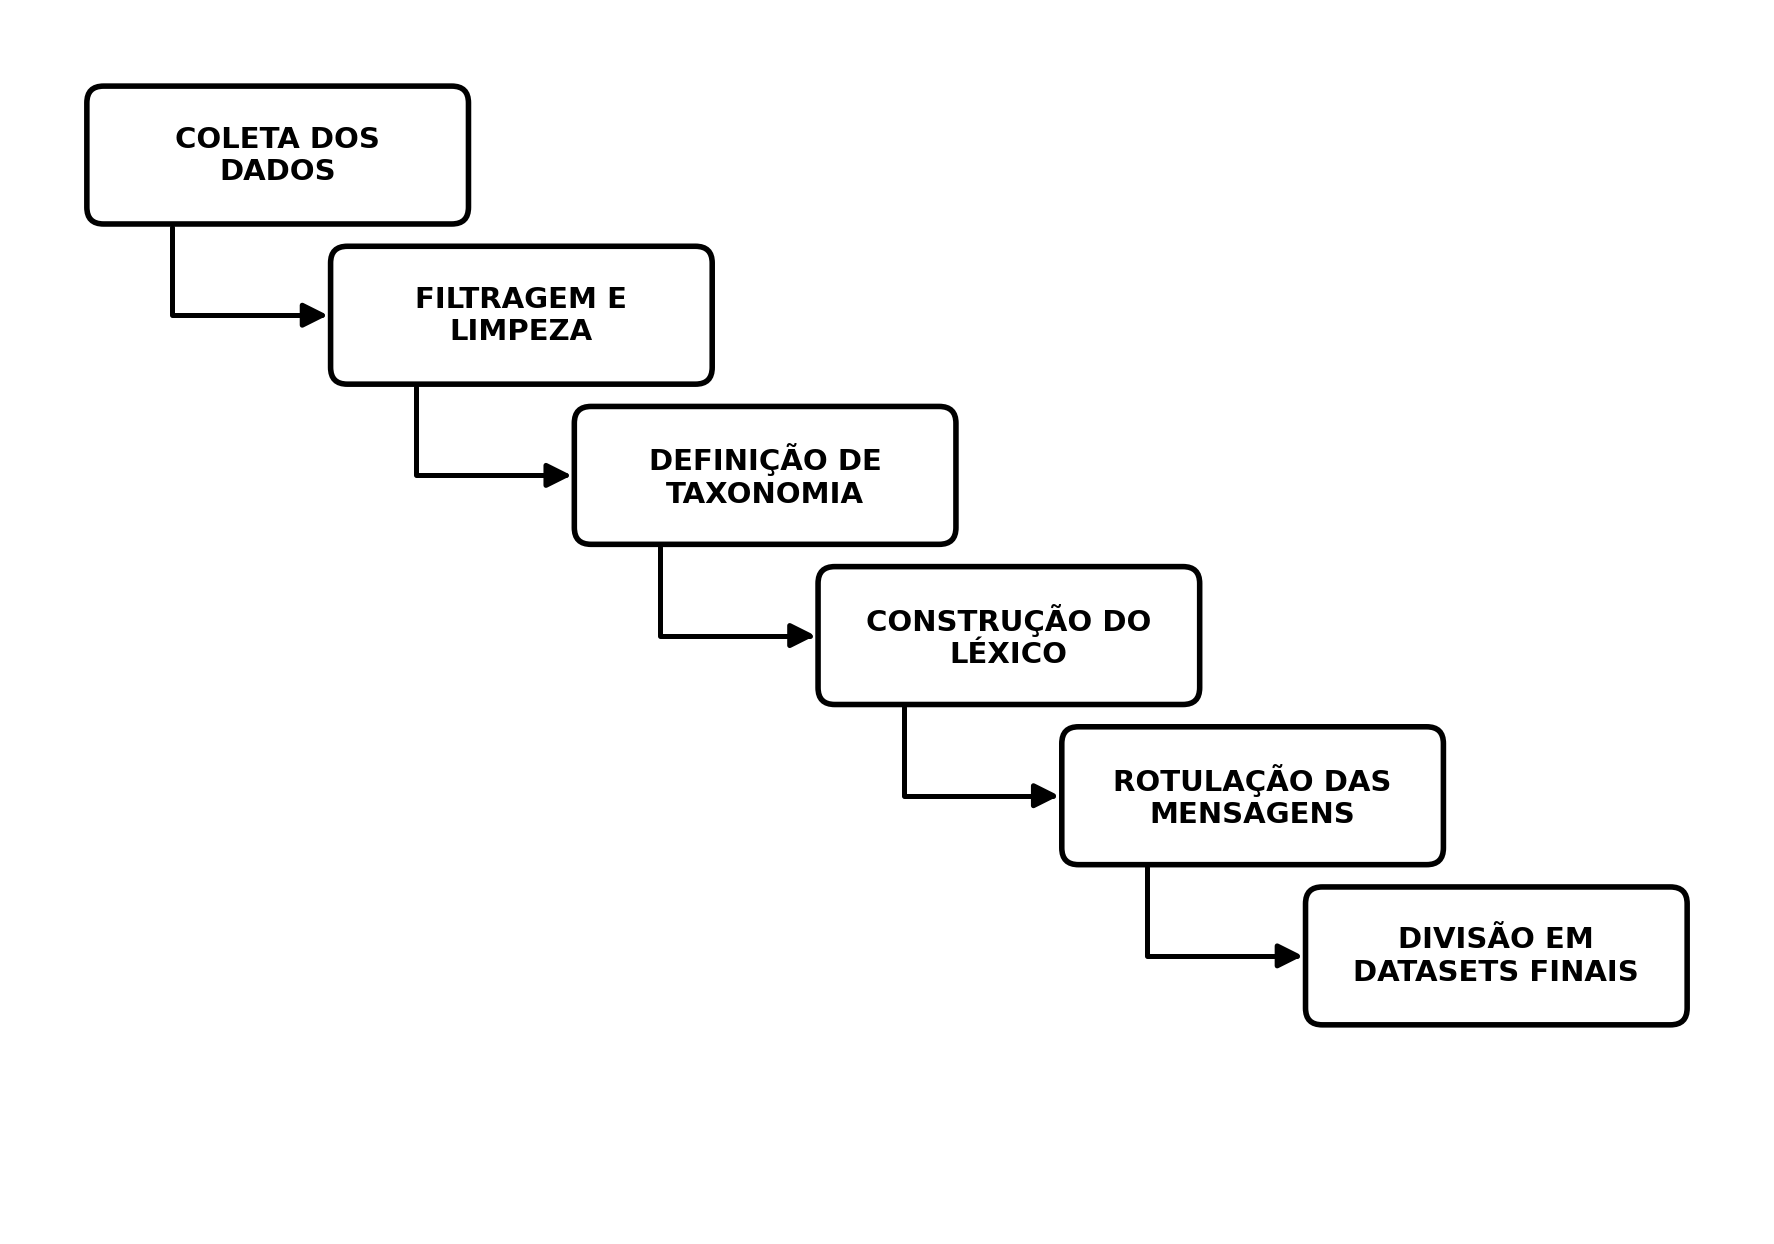
\includegraphics[width=0.85\textwidth]{figuras/fig_arquitetura.png}
    \caption{Diagrama das etapas da Modelagem da Solução}
    \label{fig:arquitetura}
\end{figure}


A modelagem apresentada estabelece a arquitetura geral da solução e evidencia a forma como os módulos se integram ao longo do desenvolvimento do trabalho. Conforme sintetizado na Figura~\ref{fig:arquitetura}, as etapas representam o encadeamento lógico das atividades planejadas e executadas até o momento. Cada decisão técnica foi concebida de modo a permitir que o sistema opere de forma eficiente sobre a linguagem \textit{gamer} brasileira, preservando simultaneamente princípios éticos, consistência metodológica e viabilidade computacional.

\section{Construção da Solução}

A construção da solução foi realizada em duas frentes principais: o desenvolvimento de uma ferramenta de coleta automatizada de mensagens da Twitch e a implementação de um \textit{pipeline} de limpeza e consolidação dos dados obtidos.

Para a coleta de dados na plataforma Twitch, foi desenvolvido um \textit{scraper} em Node.js utilizando a biblioteca \textit{tmi.js}\footnote{https://tmijs.com/}, que permite conexão autenticada ao \textit{chat} ao vivo de canais. A ferramenta verifica automaticamente se cada canal da lista está em transmissão ao vivo e, em caso positivo, conecta-se ao \textit{chat} e registra todas as mensagens por até uma hora, armazenando-as em arquivos CSV individuais por canal e data. Cada registro contém as colunas: \textit{timestamp}, \textit{channel}, \textit{username}, \textit{display\_name}, \textit{color}, \textit{badges} e \textit{message}.

Foram configurados 49 canais de \textit{streamers} brasileiros para monitoramento, cobrindo diferentes perfis de conteúdo: \textit{streamers} especializados em League of Legends (baiano, brtt, coreano, rakin e o canal oficial CBLOL), em CS2 e jogos FPS (burgaofps, fnxlntc, fer e gaules), e \textit{streamers} de variedade com grandes audiências (cellbit, alanzoka, gabepeixe, snopey, tck10, sacy, loud\_coringa, entre outros).Os endereços dos canais citados nominalmente neste trabalho estão listados no Apêndice~\ref{apendice:canais}. As coletas foram realizadas entre abril e junho de 2026, gerando centenas de arquivos CSV individuais a partir dos 30 canais que estiveram ao vivo durante os períodos de monitoramento.

O volume bruto coletado, da ordem de 1,2 milhão de mensagens, foi processado pelo \textit{script} \textit{filter\_and\_merge.py}, desenvolvido em Python com o auxílio da biblioteca \textit{pandas}. Esse \textit{pipeline} de limpeza aplica filtros sequenciais para remover conteúdo que não representa comunicação humana genuína: mensagens automatizadas do \textit{broadcaster} (avisos de inscrição, anúncios de patrocinadores), bots conhecidos (identificados por lista e por padrão de nome), comandos de \textit{chat} (mensagens iniciadas por \texttt{!}, \texttt{/} ou \texttt{.}), \textit{spam} e propaganda (URLs, menções a canais externos, mensagens com alto índice de letras maiúsculas) e, por fim, duplicatas. A Figura~\ref{fig:pipeline-limpeza} resume o efeito cumulativo de cada etapa sobre o volume do corpus.

O filtro de \textit{spam} concentra a maior parte da redução, o que é esperado em \textit{chats} de grande audiência, onde mensagens repetidas em massa (\textit{copypastas}, campanhas de doação e \textit{raids} de outros canais) são um padrão recorrente. A etapa de deduplicação foi refinada nesta fase do trabalho para também capturar quase-duplicatas — a mesma combinação de canal, usuário e mensagem reenviada em um intervalo de poucos segundos, um artefato comum de problemas de conexão do cliente de \textit{chat}. Uma primeira tentativa de generalizar esse filtro para qualquer frase repetida em excesso revelou-se inadequada: ela também descartava \textit{spam} de emotes, um padrão linguístico legítimo e amplamente aceito na cultura da Twitch. A solução adotada foi mais conservadora direcionada às contas identificadas como responsáveis pelo comportamento indevido, evitando o risco de remover interações autênticas da comunidade.

\begin{figure}[htb]
    \centering
    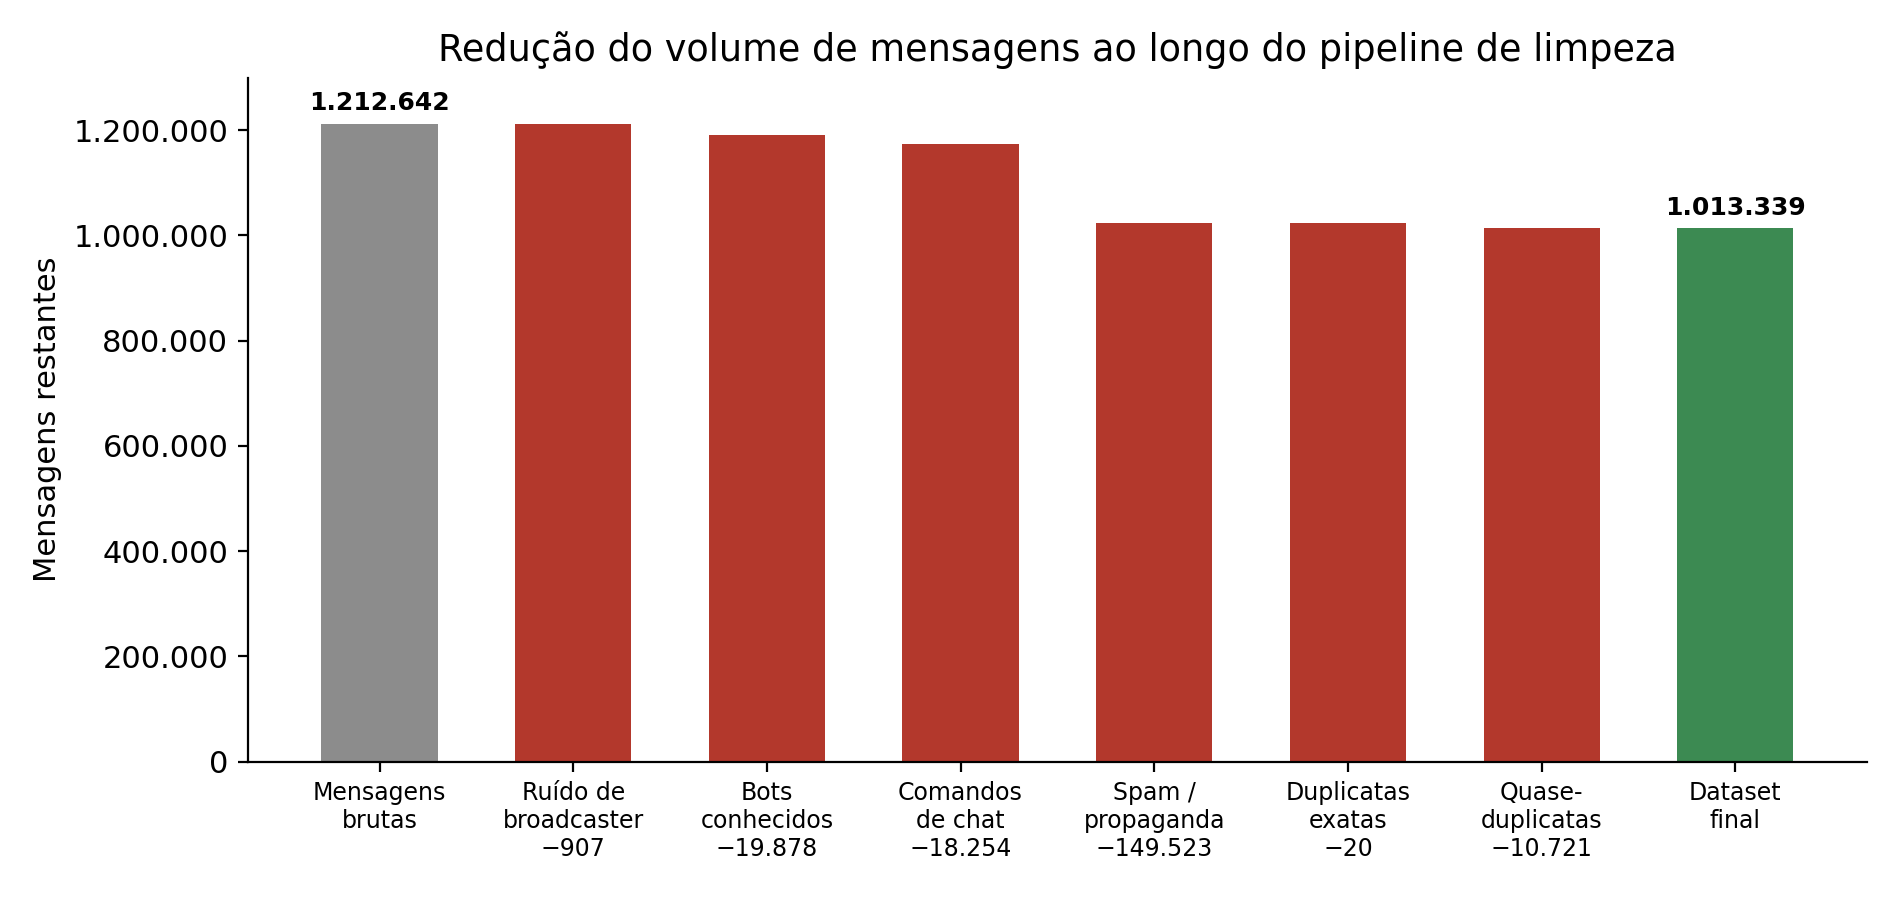
\includegraphics[width=\textwidth]{figuras/fig_pipeline_limpeza.png}
    \caption{Redução do volume de mensagens ao longo do pipeline de limpeza}
    \label{fig:pipeline-limpeza}
\end{figure}

Após a aplicação do \textit{pipeline} de limpeza, o \textit{dataset} consolidado contém \textbf{1.013.339 mensagens} distribuídas entre os 30 canais monitorados, armazenadas no arquivo \textit{final\_chat.csv}. A Tabela~\ref{tab:streamers} apresenta os maiores contribuidores em volume de mensagens.

\begin{table}[h!]
\centering
\small
\begin{tabular}{llr}
\hline
\textbf{Canal} & \textbf{Tipo de Conteúdo} & \textbf{Mensagens} \\ \hline
cellbit          & Variedade         & 215.996 \\
tck10            & Variedade         & 105.433 \\
snopey           & Variedade         & 102.283 \\
gabepeixe        & Variedade         & 100.256 \\
alanzoka         & Variedade         &  87.954 \\
sacy             & Variedade         &  55.756 \\
rakin            & League of Legends &  55.356 \\
skipnho          & Variedade         &  41.270 \\
zagowt           & Variedade         &  39.249 \\
loud\_coringa    & Variedade         &  32.242 \\
coreano          & League of Legends &  29.526 \\
piuzinho         & Variedade         &  26.707 \\
baiano           & League of Legends &  23.871 \\
frttt            & Variedade         &  18.226 \\
burgaofps        & CS2               &  13.744 \\
Demais (15)      & ---                &  65.470 \\ \hline
\textbf{Total}   &                   & \textbf{1.013.339} \\ \hline
\end{tabular}
\caption{Distribuição de mensagens por canal no \textit{dataset} final}
\label{tab:streamers}
\end{table}

O \textit{dataset} resultante constitui a principal contribuição deste trabalho, oferecendo uma base de dados especializada em português brasileiro, representativa da linguagem utilizada em comunidades \textit{gamer}, com diversidade de jogos, perfis de \textit{streamers} e períodos de coleta.

\subsection{Construção do Léxico e Rotulação Automática}
\label{sec:lexico}

Para viabilizar a rotulação do \textit{dataset} dentro do prazo do TCC II, optou-se por uma abordagem automática baseada em léxico e regras, em vez de anotação manual ou assistida por \textit{LLM}, dado o volume de mais de 1 milhão de mensagens. Essa abordagem reaproveita e formaliza, como recurso reutilizável, o segundo \textit{dataset} de gírias e termos ofensivos já previsto entre os objetivos do trabalho (Seção~\ref{sec:objetivos}).

O léxico foi estruturado em um único arquivo \textit{lexicon/lexicon.csv}, com colunas \textit{term} (forma normalizada do termo), \textit{category} (GIRIA, INS, DO, OBS ou AME), \textit{type} (\textit{word} para termos diretos, \textit{word\_ambiguous} para termos que só são ofensivos quando combinados a um marcador de direcionamento, ou \textit{phrase\_pattern} para padrões de frase em expressão regular) e \textit{notes}. Ao longo do desenvolvimento, o conjunto inicial foi substancialmente ampliado e hoje reúne mais de 500 entradas, com predominância de gírias \textit{gamer} neutras (ex.: \textit{gg}, \textit{noob}, \textit{feed}, \textit{smurf}, \textit{clutch}, \textit{tilt}) e cobertura mais ampla das categorias de insulto, discurso de ódio, obscenidade e ameaça. A expansão incorporou variações morfológicas comuns na linguagem informal do \textit{chat} — diminutivos e aumentativos, grafias alternativas e normalização de \textit{leetspeak} (substituição de letras por números, como em \textit{m4c4c0}) —, de modo que o léxico reconheça a mesma ofensa independentemente de pequenas variações ortográficas. Termos ambíguos no vocabulário \textit{gamer} — como \textit{noob}, \textit{bot}, \textit{hacker}, \textit{cheater} e \textit{trash} — aparecem simultaneamente como gíria neutra e como insulto condicional: só contam como insulto quando a mensagem também contém uma menção (\texttt{@usuário}) ou pronome de segunda pessoa, distinguindo \textit{"deu um bot ali"} (neutro) de \textit{"@user vc é bot"} (ofensivo). Os termos de discurso de ódio foram curados com referência aos critérios discutidos na Fundamentação Teórica (Seção~\ref{sec:taxonomia}), tomando como inspiração as categorias do ToLD-BR \cite{ricarte2025contextual} e do HateBR \cite{vargas2022hatebr}, e devem ser entendidos como um conjunto extensível, não exaustivo.

O \textit{script} \textit{annotate.py}, desenvolvido em Python com \textit{pandas} no mesmo estilo do \textit{filter\_and\_merge.py}, implementa a rotulação em duas etapas. Primeiro, a mensagem é normalizada (conversão para minúsculas e remoção de acentos) e comparada contra o léxico de forma vetorizada: insultos, discurso de ódio e obscenidade são detectados pela presença de termos (com tratamento especial para termos curtos, que exigem correspondência exata, evitando que prefixos como \textit{bot} casem com palavras não relacionadas como \textit{bota}); ameaças são detectadas pelos padrões de frase; e assédio é calculado por uma heurística composta — agrupando mensagens por canal, remetente e alvo mencionado, e marcando como assédio as rajadas em que o mesmo remetente direciona um termo ofensivo (insulto ou discurso de ódio) ao mesmo alvo três ou mais vezes dentro de uma janela de cinco minutos, parâmetros configuráveis via linha de comando. Menções (\texttt{@usuário}) são mascaradas antes da busca lexical em nível de sentença, evitando falsos positivos quando o nome de um usuário ou \textit{streamer} contém, por coincidência, uma substring presente no léxico. Em seguida, cada mensagem é tokenizada e cada \textit{token} recebe um rótulo (TÓXICO, GÍRIA\_GAMER ou NEUTRO), serializado como uma lista de pares \textit{token}–rótulo em formato JSON na coluna \textit{token\_labels} — opção mais simples do que o formato BIO usado em tarefas de reconhecimento de entidades, já que os três rótulos não exigem marcação de fronteiras de \textit{spans} multi-\textit{token}.

A execução do script sobre o corpus de 1.013.339 mensagens produziu o arquivo \textit{final\_chat\_labeled.csv}, cujos resultados quantitativos são apresentados na Seção~\ref{sec:distribuicao-rotulos}.

\chapter{Caracterização do Dataset}
\label{cha:caracterizacao}

\section{Perfil do Corpus}

Cada entrada do \textit{dataset} contém os campos apresentados na Tabela~\ref{tab:colunas}, que permitem identificar o contexto da mensagem, o usuário que a enviou e o canal em que ocorreu a interação.

\begin{table}[h!]
\centering
\small
\begin{tabular}{ll}
\hline
\textbf{Campo} & \textbf{Descrição} \\ \hline
\textit{timestamp}     & Data e hora de envio da mensagem (UTC) \\
\textit{channel}       & Nome do canal da Twitch onde a mensagem foi enviada \\
\textit{username}      & Nome de usuário do remetente \\
\textit{display\_name} & Nome de exibição do remetente \\
\textit{color}         & Cor do nome do usuário no \textit{chat} \\
\textit{badges}        & Insígnias do usuário (ex.: \textit{subscriber}, \textit{moderator}) \\
\textit{message}       & Texto da mensagem enviada \\ \hline
\end{tabular}
\caption{Campos do \textit{dataset} final}
\label{tab:colunas}
\end{table}

O \textit{dataset} cobre uma ampla variedade de contextos dentro do universo \textit{gamer} brasileiro. Os canais coletados incluem \textit{streamers} de jogos competitivos, como League of Legends e CS2, e \textit{streamers} de variedade com grandes audiências. Essa diversidade é importante para que o corpus represente diferentes registros linguísticos, vocabulários específicos de cada jogo e dinâmicas de \textit{chat} distintas.

Embora o GameTox \cite{naseem-etal-2025-gametox} tenha sido anotado manualmente, enquanto a rotulação deste corpus é automática, baseada em léxico e regras (Seção~\ref{sec:lexico}) — de modo que os dois recursos não são diretamente comparáveis em termos de qualidade dos rótulos —, o \textit{dataset} aqui construído se destaca em termos de volume e especialização linguística: reúne mais de 1 milhão de mensagens em português brasileiro, abrangendo múltiplos jogos e diferentes perfis de \textit{streamers}, frente às 53 mil mensagens de um único jogo (\textit{World of Tanks}) em inglês do GameTox.

\section{Exportações Derivadas}
\label{sec:exportacoes}

A partir do \textit{dataset} rotulado, foram gerados artefatos auxiliares que facilitam o consumo dos dados para diferentes finalidades de pesquisa. O \textit{script} \textit{export\_toxic.py} separa o corpus em dois arquivos — mensagens tóxicas e não tóxicas —, descartando deste último as mensagens compostas exclusivamente por risadas (ex.: \textit{"kkkkk"}), que não carregam conteúdo linguístico relevante para tarefas de classificação. De forma semelhante, o \textit{script} \textit{export\_girias.py} produz um arquivo com uma ocorrência por linha de cada gíria identificada no corpus, também excluindo risadas do conceito de gíria.

O \textit{script} \textit{toxicity\_by\_stream.py} calcula a taxa de toxicidade por canal, permitindo comparar o comportamento das diferentes comunidades monitoradas. Para cada canal, essa taxa é calculada como a proporção entre a quantidade de mensagens classificadas como tóxicas (em qualquer uma das categorias da Tabela~\ref{tab:taxonomia}) e o total de mensagens coletadas daquele mesmo canal durante o período observado nesta pesquisa. Por exemplo, o canal \textit{loud\_coringa} registrou 527 mensagens tóxicas entre as 32.272 mensagens coletadas dele no período monitorado, resultando em uma taxa de 1,63\%: ou seja, das mensagens desse canal, 1,63\% foram tóxicas e 98,37\% não tóxicas. A Figura~\ref{fig:ranking-canais} apresenta os canais com maior e menor taxa de mensagens tóxicas entre os que tiveram volume suficiente para uma estimativa confiável. A variação observada entre canais — de menos de 1\% a mais de 7\% de mensagens tóxicas — sugere que o perfil do \textit{streamer} e da comunidade que se forma em torno dele tem efeito relevante sobre o nível de toxicidade do \textit{chat}, uma hipótese que pode ser explorada em trabalhos futuros.

\begin{figure}[H]
    \centering
    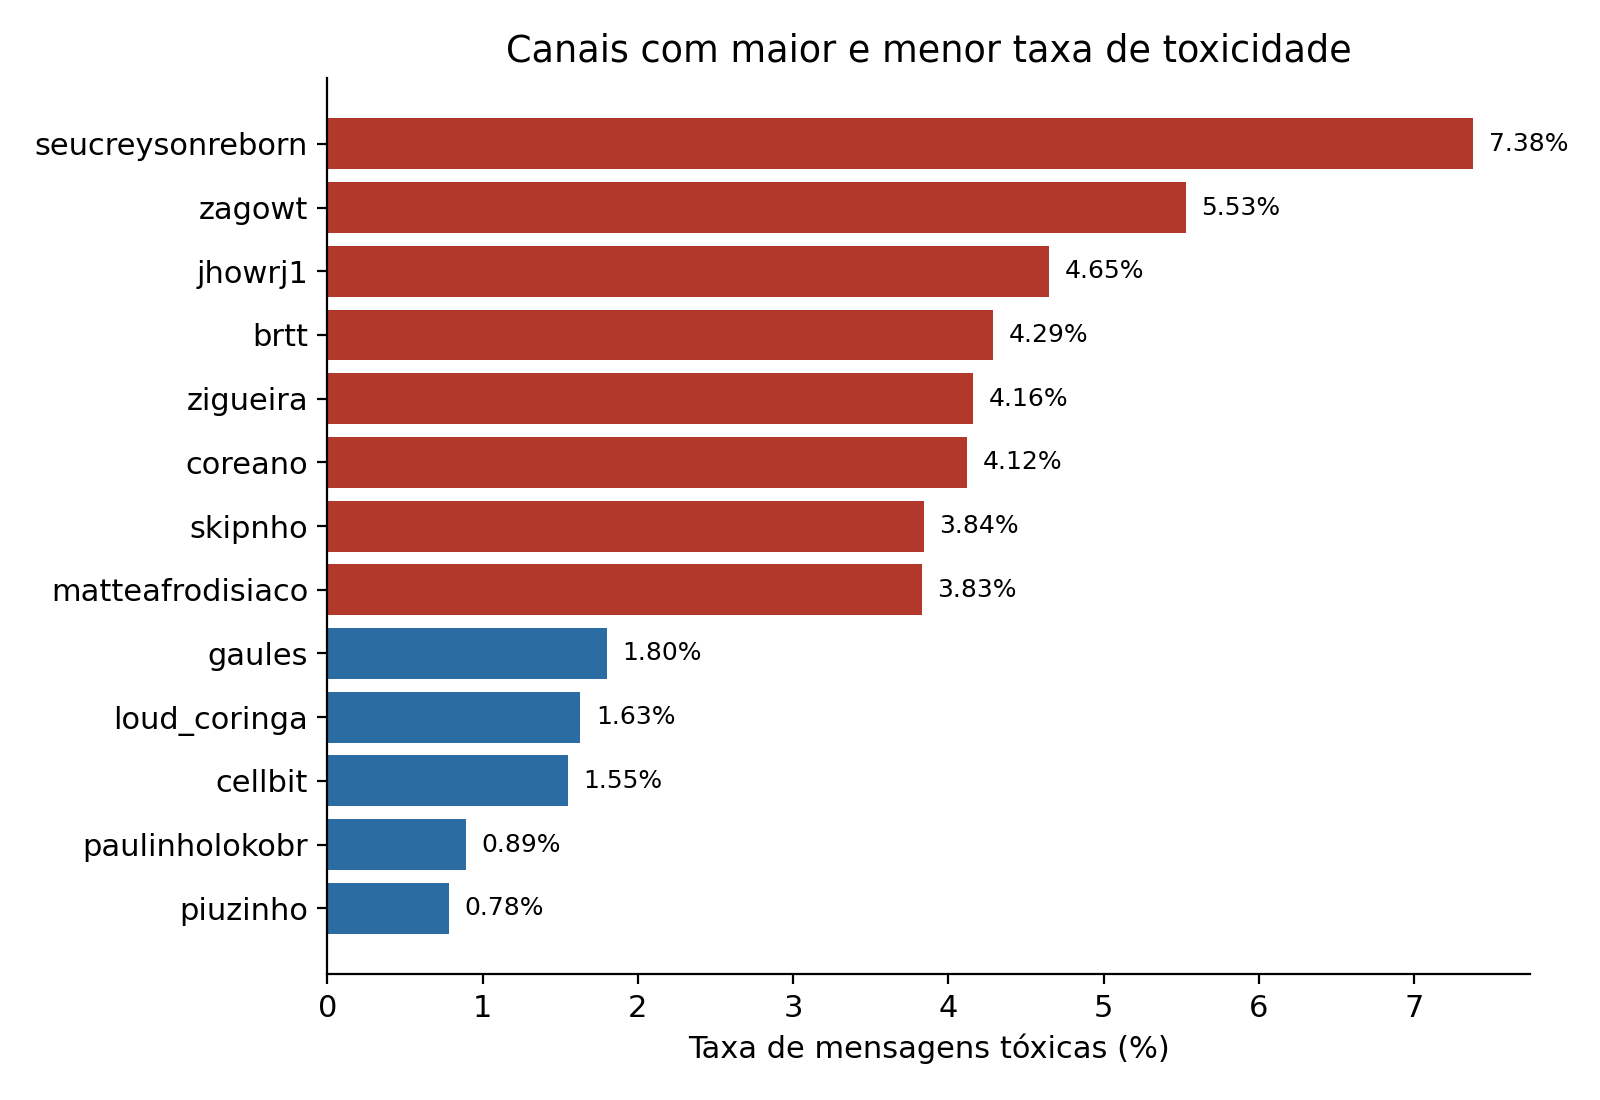
\includegraphics[width=0.9\textwidth]{figuras/fig_ranking_canais.png}
    \caption{Canais com maior e menor taxa de toxicidade}
    \label{fig:ranking-canais}
\end{figure}

\section{Auditoria de Qualidade}

Para validar a integridade do processo de deduplicação, foi desenvolvido o \textit{script} \textit{check\_duplicates.py}, que investiga ocorrências de mensagens aparentemente repetidas nos artefatos exportados. A auditoria identificou que a maior parte dessas ocorrências reflete apenas a perda de granularidade dos arquivos de exportação — que não preservam usuário e horário exatos — e não duplicação real dos dados. Já as duplicatas técnicas genuínas, isto é, a mesma combinação de canal, usuário e mensagem reenviada em poucos segundos, encontram-se hoje eliminadas pelo filtro de quase-duplicatas incorporado ao \textit{pipeline} de limpeza (Seção~\ref{cha:desenvolvimento}).

\section{Distribuição dos Rótulos}
\label{sec:distribuicao-rotulos}

Conforme descrito na Seção~\ref{sec:lexico}, o \textit{dataset} foi rotulado automaticamente por meio de léxico e regras, seguindo a taxonomia da Seção~\ref{sec:taxonomia}. A Figura~\ref{fig:distribuicao-sentenca} e a Tabela~\ref{tab:distribuicao_sentenca} apresentam a distribuição das mensagens nas seis categorias de sentença. Como o esquema é multi-rótulo — inspirado no ToLD-BR —, uma mesma mensagem pode pertencer a mais de uma categoria simultaneamente, o que ocorreu em uma pequena fração das mensagens tóxicas.

\begin{figure}[htb]
    \centering
    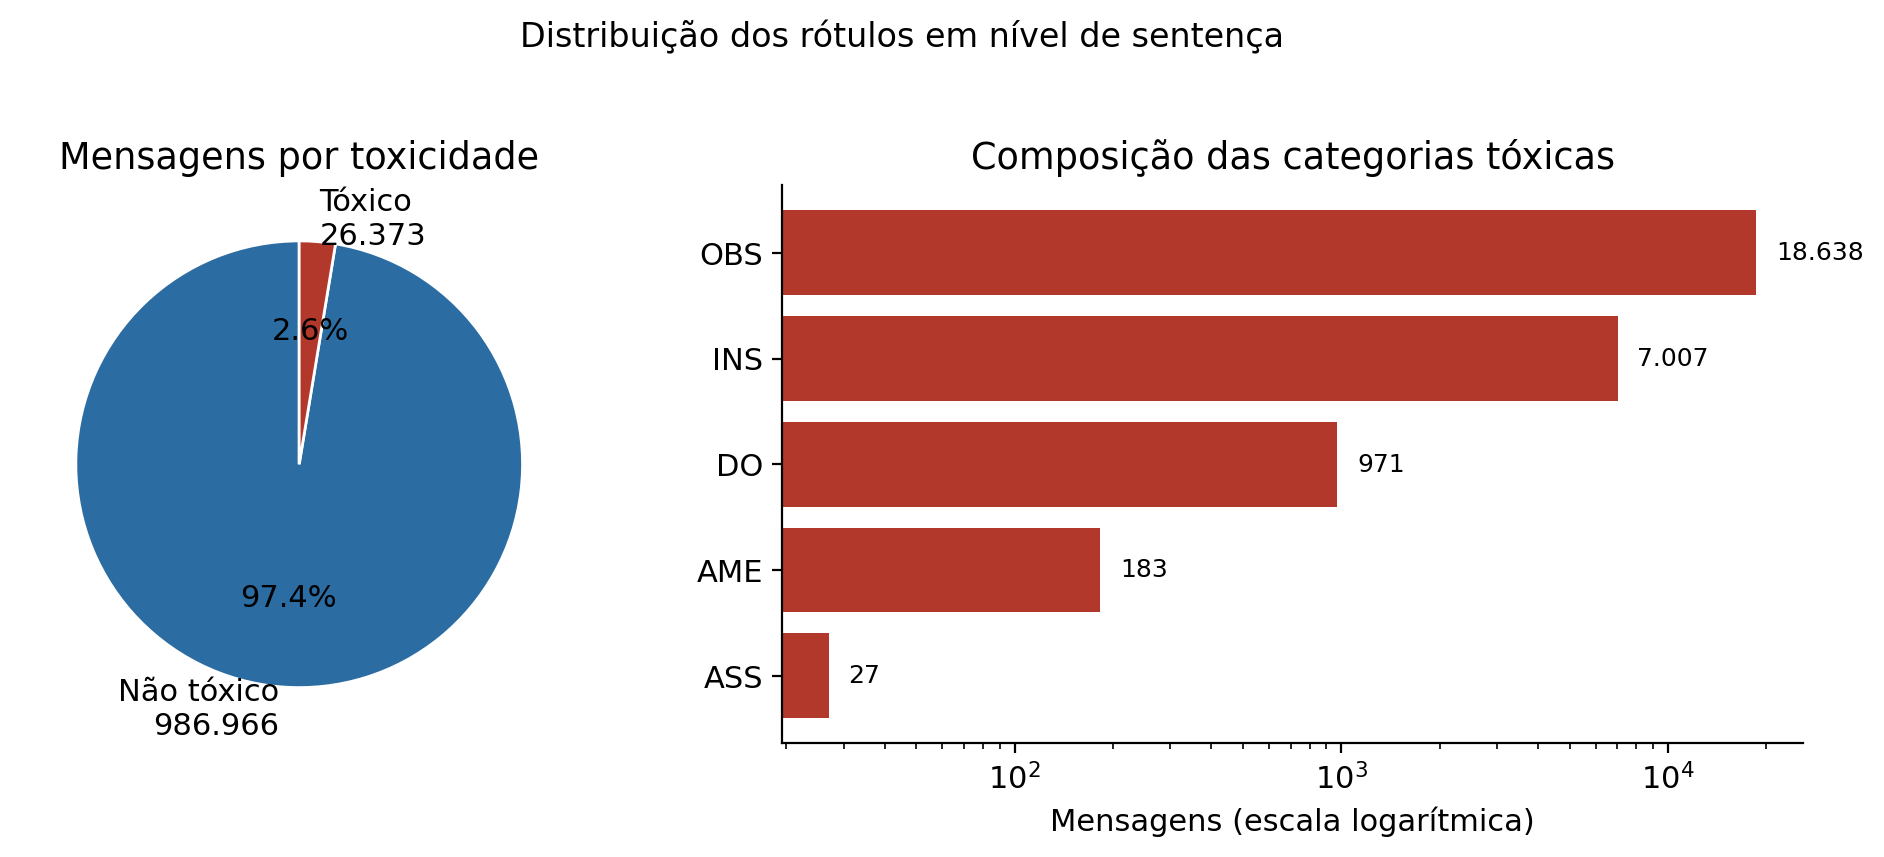
\includegraphics[width=\textwidth]{figuras/fig_distribuicao_sentenca.png}
    \caption{Distribuição dos rótulos em nível de sentença}
    \label{fig:distribuicao-sentenca}
\end{figure}

\begin{table}[h!]
\centering
\small
\begin{tabular}{lrr}
\hline
\textbf{Categoria} & \textbf{Mensagens} & \textbf{Percentual} \\ \hline
Não Tóxico (NT)        & 986.966 & 97,40\% \\
Insulto (INS)           &   7.007 &  0,69\% \\
Assédio (ASS)           &      27 &  0,00\% \\
Discurso de Ódio (DO)   &     971 &  0,10\% \\
Ameaça (AME)            &     183 &  0,02\% \\
Obscenidade (OBS)       &  18.638 &  1,84\% \\ \hline
\textbf{Total de mensagens} & \textbf{1.013.339} & \\
\textbf{Mensagens tóxicas (qualquer categoria $\neq$ NT)} & \textbf{26.373} & \textbf{2,60\%} \\ \hline
\end{tabular}
\caption{Distribuição das mensagens por categoria de toxicidade (nível de sentença)}
\label{tab:distribuicao_sentenca}
\end{table}

O baixo percentual de mensagens tóxicas é consistente com o desbalanceamento entre classes tóxicas e não tóxicas relatado na literatura sobre \textit{datasets} de discurso de ódio \cite{madukwe2022token}, reforçando a necessidade de técnicas de balanceamento em eventuais etapas futuras de treinamento supervisionado. A obscenidade é, isoladamente, a categoria mais frequente, em boa parte por capturar palavrões de uso amplamente coloquial no português brasileiro, que funcionam como interjeição de ênfase e nem sempre indicam toxicidade real — uma limitação discutida no Capítulo~\ref{cha:conclusao}. Já assédio e ameaça são as categorias mais raras, o que é esperado dado o caráter mais restritivo das heurísticas utilizadas para identificá-las.

A Figura~\ref{fig:distribuicao-token} e a Tabela~\ref{tab:distribuicao_token} apresentam a distribuição em nível de \textit{token}, calculada sobre o conjunto de \textit{tokens} extraídos do corpus.

\begin{figure}[htb]
    \centering
    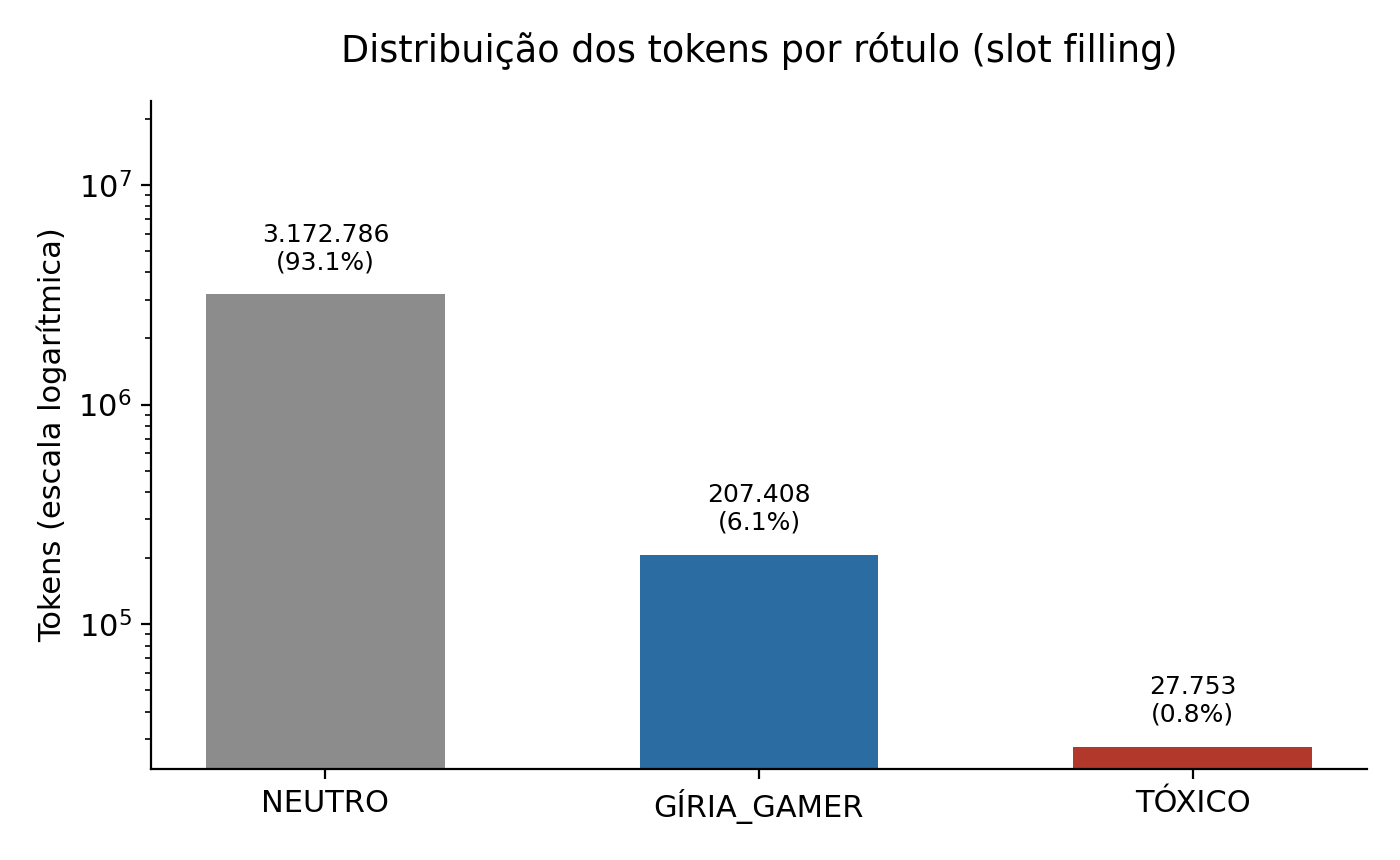
\includegraphics[width=0.75\textwidth]{figuras/fig_distribuicao_token.png}
    \caption{Distribuição dos tokens por rótulo (slot filling)}
    \label{fig:distribuicao-token}
\end{figure}

\begin{table}[h!]
\centering
\small
\begin{tabular}{lrr}
\hline
\textbf{Rótulo} & \textbf{Tokens} & \textbf{Percentual} \\ \hline
NEUTRO       & 3.172.786 & 93,10\% \\
GÍRIA\_GAMER &   207.408 &  6,09\% \\
TÓXICO       &    27.753 &  0,81\% \\ \hline
\textbf{Total} & \textbf{3.407.947} & \\ \hline
\end{tabular}
\caption{Distribuição dos tokens por rótulo (nível de slot filling)}
\label{tab:distribuicao_token}
\end{table}

A proporção de gírias \textit{gamer} em nível de \textit{token} (6,09\%) é bem superior à de \textit{tokens} tóxicos (0,81\%), reforçando que o vocabulário desse universo é majoritariamente composto por jargão neutro de jogo, e não por ofensas. Essa distinção é justamente o que motiva a anotação em dois níveis adotada neste trabalho: ela permite que modelos futuros aprendam a diferenciar gíria de toxicidade, em vez de tratar todo vocabulário não convencional como sinal de agressividade.

\section{Nuvens de Palavras}
\label{sec:nuvens-palavras}

Como complemento qualitativo à distribuição quantitativa apresentada na Seção~\ref{sec:distribuicao-rotulos}, foram geradas nuvens de palavras a partir dos termos mais frequentes em cada um dos três conjuntos de exportação descritos na Seção~\ref{sec:exportacoes}: mensagens não tóxicas, gírias \textit{gamer} e mensagens tóxicas. As Figuras~\ref{fig:nuvem-neutras}, \ref{fig:nuvem-girias} e \ref{fig:nuvem-toxicas} ilustram, respectivamente, os termos predominantes em cada conjunto, com o tamanho de cada palavra proporcional à sua frequência de ocorrência. A Tabela~\ref{tab:contagem_palavras} apresenta o quantitativo que fundamenta essas nuvens, com os dez termos mais frequentes de cada categoria.

\begin{figure}[htb]
    \centering
    \begin{subfigure}[b]{0.32\textwidth}
        \centering
        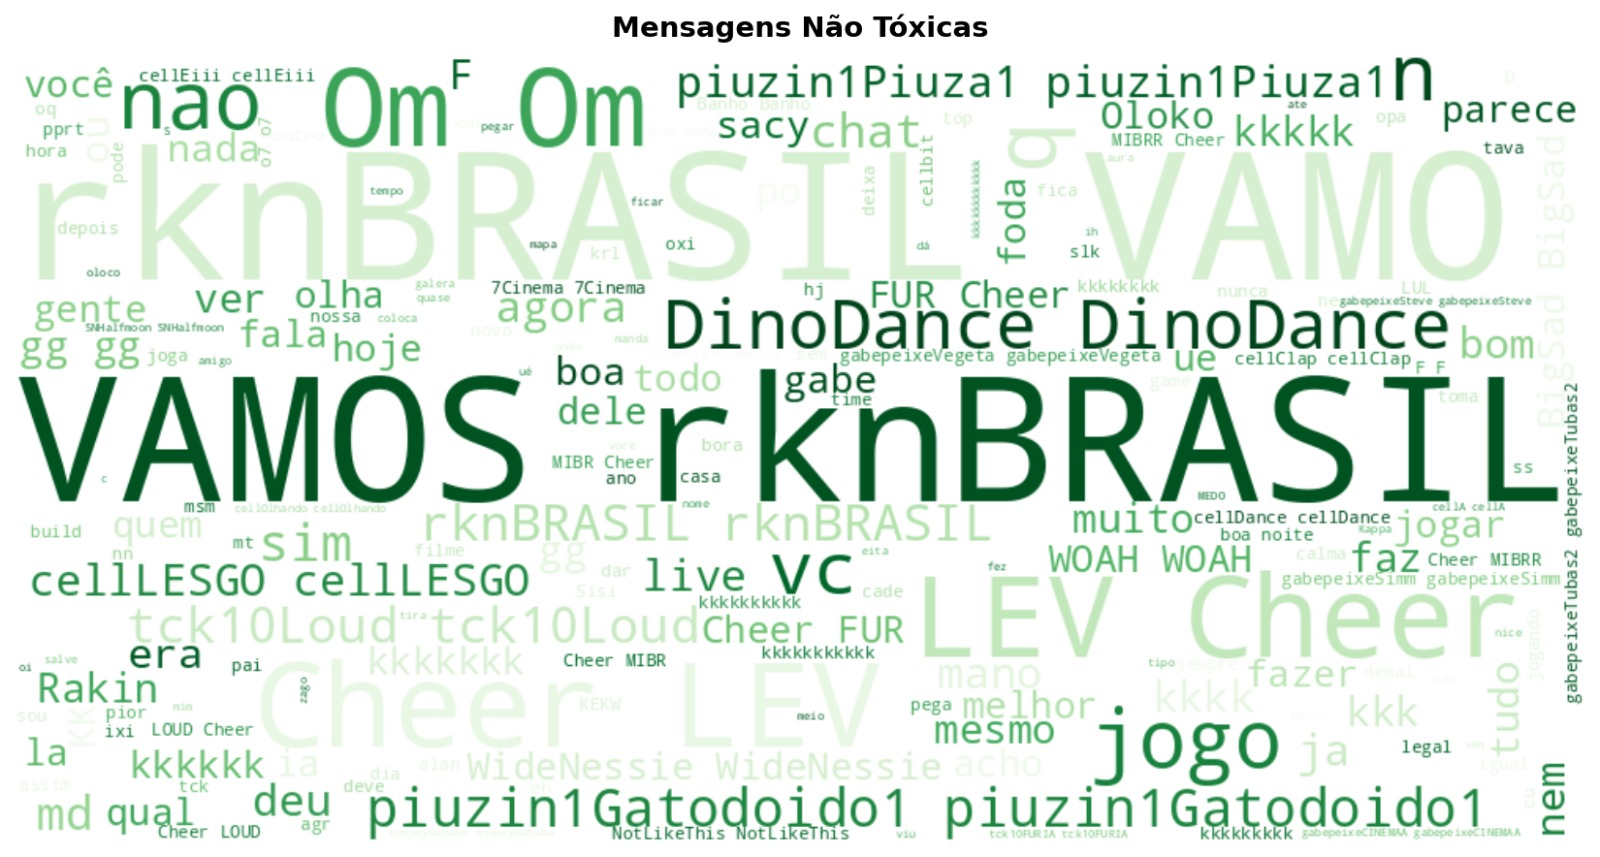
\includegraphics[width=\textwidth]{figuras/fig_nuvem_neutras.jpeg}
        \caption{Não tóxicas}
        \label{fig:nuvem-neutras}
    \end{subfigure}
    \hfill
    \begin{subfigure}[b]{0.32\textwidth}
        \centering
        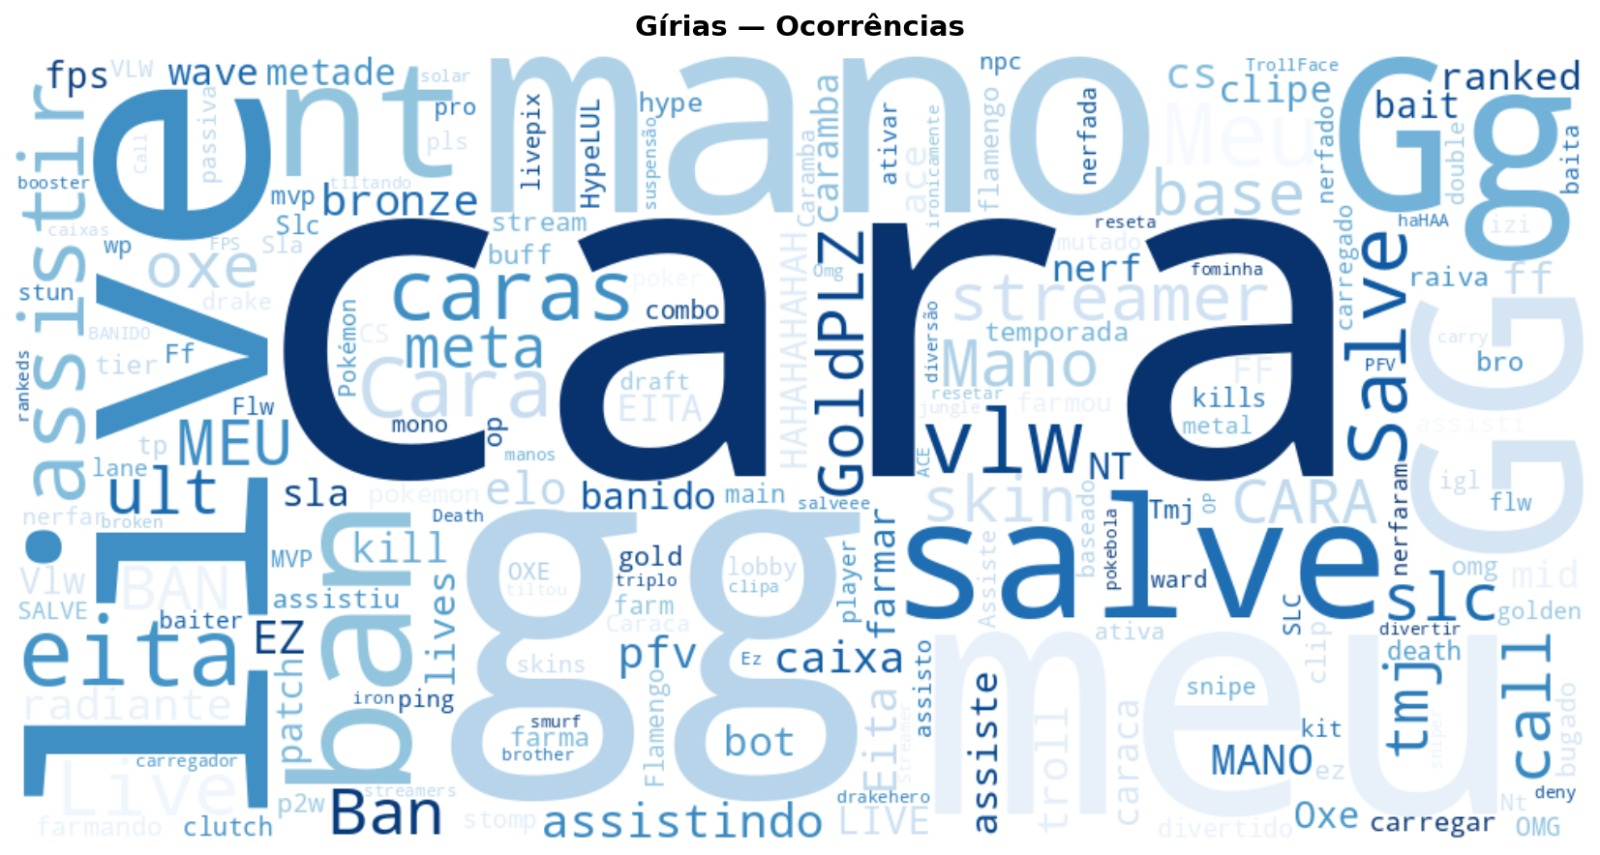
\includegraphics[width=\textwidth]{figuras/fig_nuvem_girias.jpeg}
        \caption{Gírias \textit{gamer}}
        \label{fig:nuvem-girias}
    \end{subfigure}
    \hfill
    \begin{subfigure}[b]{0.32\textwidth}
        \centering
        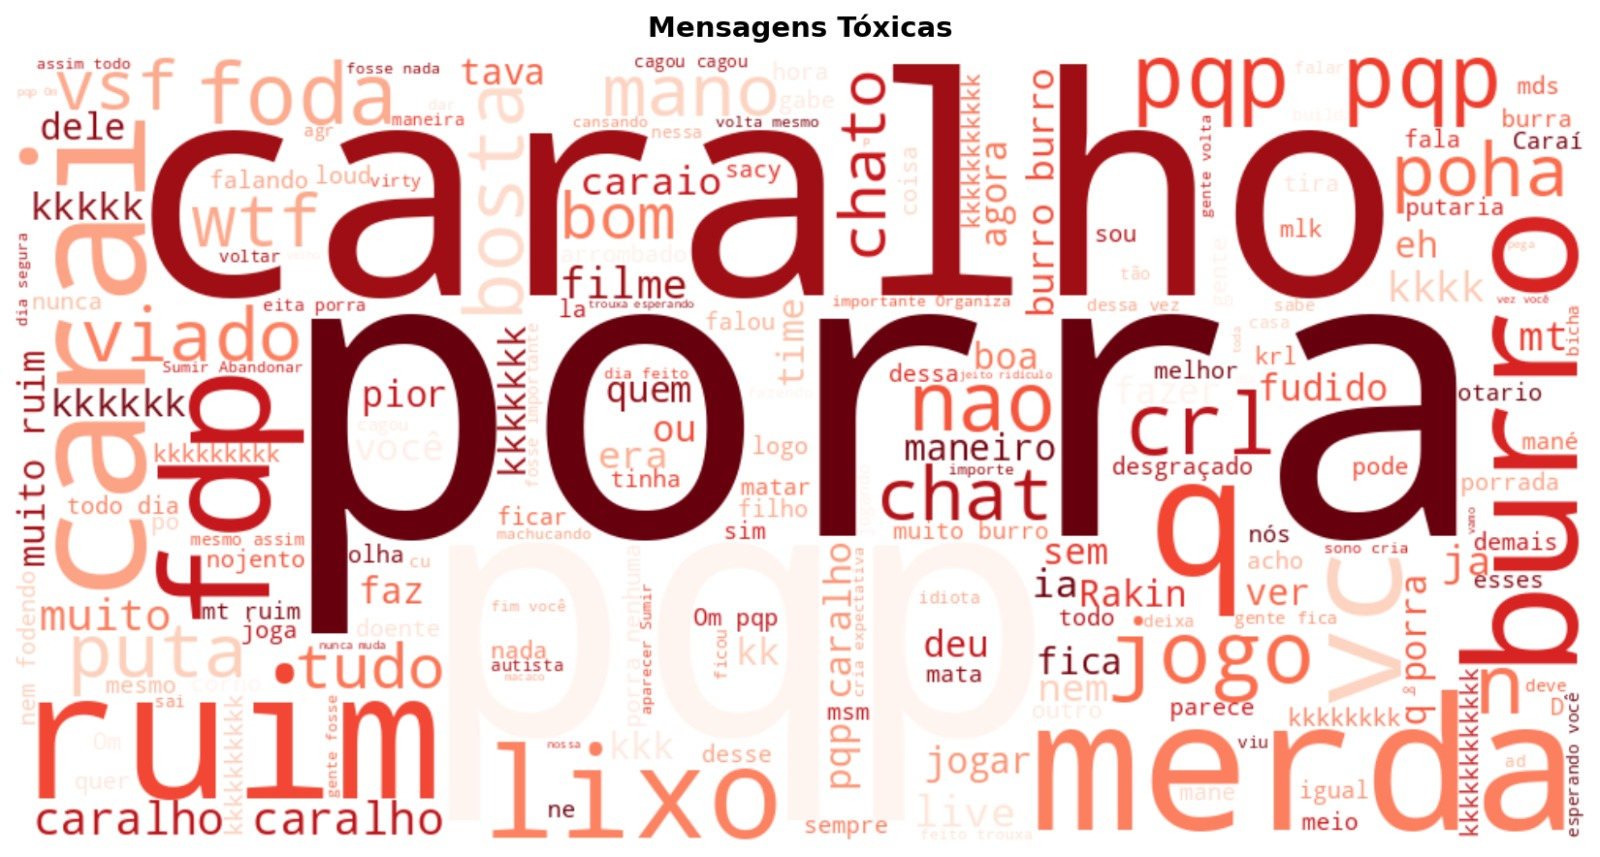
\includegraphics[width=\textwidth]{figuras/fig_nuvem_toxicas.jpeg}
        \caption{Tóxicas}
        \label{fig:nuvem-toxicas}
    \end{subfigure}
    \caption{Nuvens de palavras por tipo de mensagem}
    \label{fig:nuvens-palavras}
\end{figure}

\begin{table}[h!]
\centering
\small
\begin{tabular}{lr|lr|lr}
\hline
\multicolumn{2}{c}{\textbf{Gírias}} & \multicolumn{2}{c}{\textbf{Não tóxicas}} & \multicolumn{2}{c}{\textbf{Tóxicas}} \\ \hline
cara    & 13.601 & rknbrasil & 62.950 & porra   & 3.671 \\
gg      & 12.169 & vamos     & 54.203 & pqp     & 3.612 \\
meu     &  6.932 & om        & 38.581 & caralho & 2.377 \\
live    &  6.017 & cheer     & 27.100 & ruim    & 1.988 \\
mano    &  5.003 & lev       & 21.530 & burro   & 1.520 \\
ban     &  2.173 & não       & 12.344 & merda   & 1.499 \\
salve   &  2.009 & gg        & 12.096 & carai   &   955 \\
nt      &  1.515 & vc        & 11.654 & fdp     &   829 \\
eita    &  1.394 & sim       &  9.906 & vc      &   813 \\
vlw     &  1.013 & jogo      &  9.352 & muito   &   663 \\ \hline
\end{tabular}
\caption{Dez termos mais frequentes por categoria}
\label{tab:contagem_palavras}
\end{table}

As gírias mais frequentes, \textit{"cara"}, \textit{"gg"}, \textit{"mano"}, confirmam o caráter coloquial e de camaradagem predominante no vocabulário \textit{gamer}, conforme já discutido na Seção~\ref{sec:distribuicao-rotulos}. Entre as mensagens não tóxicas, chama atenção a presença de termos como \textit{"rknbrasil"}, \textit{"om"}, \textit{"cheer"} e \textit{"lev"}, que não são palavras do vocabulário comum, mas sim nomes de \textit{emotes} e termos associados a \textit{cheers} (doações em \textit{bits}) específicos de alguns canais; sua alta frequência indica que uma parcela do \textit{spam} de \textit{emotes} mencionado na Seção~\ref{cha:desenvolvimento} permanece no corpus após a limpeza, já que o filtro adotado foi deliberadamente conservador para não remover esse padrão legítimo da cultura da Twitch. Já entre as mensagens tóxicas, predominam palavrões genéricos (\textit{"porra"}, \textit{"pqp"}, \textit{"caralho"}, \textit{"merda"}), reforçando a observação já feita na Seção~\ref{sec:distribuicao-rotulos} de que a obscenidade captura, em boa parte, interjeições de ênfase e não necessariamente ataques direcionados.

Vale notar que o termo \textit{"vc"} aparece simultaneamente entre os mais frequentes das mensagens não tóxicas e das mensagens tóxicas. Isso ocorre porque as nuvens de palavras e a Tabela~\ref{tab:contagem_palavras} são construídas a partir do texto \textbf{completo} das mensagens de cada exportação (Seção~\ref{sec:exportacoes}), e não apenas dos \textit{tokens} que motivaram a classificação de toxicidade: uma mensagem é exportada para o conjunto de mensagens tóxicas quando contém pelo menos um termo do léxico em qualquer categoria, mas as demais palavras da mesma mensagem — incluindo termos neutros e extremamente comuns como \textit{"vc"} — são contabilizadas junto. Como \textit{"vc"} é uma das abreviações mais usadas no português informal de \textit{chat}, sua alta frequência nas mensagens não tóxicas é esperada, e sua presença nas mensagens tóxicas reflete apenas a coocorrência com outras palavras ofensivas na mesma mensagem (ex.: \textit{"@user vc é um lixo"}), e não que o termo em si tenha sido rotulado como tóxico.

\chapter{Conclusão}
\label{cha:conclusao}

Este trabalho propôs e executou a construção de um \textit{dataset} de toxicidade voltado para comunidades \textit{gamer} brasileiras, preenchendo uma lacuna identificada na literatura: a ausência de bases de dados especializadas em português brasileiro que representem a linguagem informal, repleta de gírias e expressões características dos ambientes de jogos \textit{on-line}.

Ao longo do TCC I, foram estabelecidos os fundamentos teóricos do trabalho — revisão da literatura sobre toxicidade em jogos, estudo de plataformas digitais de \textit{streaming} e comunicação associadas a jogos, e definição da taxonomia de toxicidade e do modelo de anotação. No TCC II, foram desenvolvidas e executadas as etapas práticas: a construção de um \textit{scraper} de \textit{chat} da Twitch em Node.js, o monitoramento de 49 canais de \textit{streamers} brasileiros, a coleta de dados entre abril e junho de 2026, o desenvolvimento de um \textit{pipeline} de limpeza e filtragem em Python, a construção e expansão de um léxico de termos \textit{gamer} e ofensivos, a rotulação automática do corpus segundo a taxonomia definida e, por fim, a geração de exportações derivadas e de uma auditoria de qualidade sobre os dados produzidos. O resultado final é um corpus de mais de \textbf{1 milhão de mensagens} em português brasileiro, distribuídas entre 30 canais de diferentes jogos e perfis de conteúdo, já rotulado em nível de sentença e de \textit{token}.

A principal contribuição deste trabalho é a disponibilização de um recurso especializado e rotulado para pesquisas futuras em Processamento de Linguagem Natural aplicado à detecção de toxicidade em comunidades \textit{gamer} brasileiras. O corpus construído é representativo, diversificado e de grande volume, superando em mais de uma ordem de magnitude, em número de mensagens, referências internacionais como o GameTox \cite{naseem-etal-2025-gametox}, que contém 53 mil mensagens de um único jogo em inglês — uma vantagem de escala e de especialização linguística no vocabulário \textit{gamer} brasileiro, e não de rigor de anotação, já que o GameTox conta com anotação manual validada e este trabalho emprega rotulação automática por léxico e regras — expressões regulares para identificar padrões de frase (ameaças) e uma heurística de persistência de remetente contra o mesmo alvo (assédio), ambas detalhadas na Seção~\ref{sec:lexico}. O corpus já incorpora rótulos de toxicidade em nível de sentença e de \textit{token}, obtidos por meio do léxico e das regras descritas na Seção~\ref{sec:lexico}.

Como limitação principal, a rotulação foi obtida por léxico e regras, não por anotação humana, o que impõe restrições conhecidas: a cobertura está limitada ao vocabulário presente no léxico, gerando falsos negativos para termos não previstos; heurísticas como a de assédio e de ameaça não captam sarcasmo, tom afetivo ou contexto implícito, podendo gerar falsos positivos (por exemplo, mensagens com tom de brincadeira entre fãs e \textit{streamer} foram capturadas pela heurística de persistência); e termos de baixo calão de uso coloquial, embora classificados como obscenidade pelo léxico, são amplamente empregados na linguagem informal brasileira como interjeições de ênfase, sem necessariamente indicar toxicidade — uma confirmação prática, sobre os próprios dados deste trabalho, da fragilidade de abordagens baseadas unicamente em palavras-chave isoladas já apontada por \cite{melo2025torna}. O processo de limpeza também evidenciou que filtros genéricos demais podem ser tão problemáticos quanto a ausência de filtros: uma tentativa inicial de generalizar a detecção de \textit{spam} por repetição de frases acabou capturando \textit{spam} de emotes, um padrão legítimo da cultura da Twitch, e precisou ser substituída por uma abordagem mais conservadora e direcionada. A validação humana sistemática da acurácia da rotulação automática está em andamento — o protocolo de amostragem estratificada por categoria, com anotação cega e múltiplos anotadores independentes, já foi definido e a amostra já foi extraída, restando a etapa de anotação e consolidação dos resultados. Além disso, a coleta foi realizada exclusivamente na Twitch, não abrangendo outras plataformas \textit{gamer} previstas na etapa de planejamento do trabalho, cuja exploração é discutida na Seção~\ref{sec:trabalhos-futuros}. Outra limitação relevante é a concentração do corpus em poucos canais: conforme a Tabela~\ref{tab:streamers}, os cinco maiores canais (cellbit, tck10, snopey, gabepeixe e alanzoka) respondem, juntos, por mais de 50\% das mensagens coletadas, todos eles \textit{streamers} de variedade de grande audiência. Isso restringe a representatividade do termo "comunidades \textit{gamer} brasileiras" adotado no título: o perfil do corpus captura fortemente o registro linguístico desse tipo de canal, podendo sub-representar comunidades menores, de jogos específicos ou de outros perfis de audiência. Por fim, a coleta de mensagens públicas de \textit{chat} não foi acompanhada de um procedimento de anonimização dos identificadores de usuário, o que deve ser tratado antes de qualquer divulgação ampla do \textit{dataset} como recurso público.

\section{Trabalhos Futuros}
\label{sec:trabalhos-futuros}

Com a rotulação automática já realizada, as próximas etapas naturais deste trabalho passam a ser: (1) a conclusão da validação humana de uma amostra estratificada dos rótulos atribuídos automaticamente — protocolo já definido e amostragem já realizada, com anotação cega e múltiplos anotadores independentes —, permitindo estimar a precisão, a cobertura do léxico e a concordância entre rotulação automática e humana frente a um padrão de referência anotado manualmente; (2) a expansão contínua do léxico, incorporando gírias regionais, termos associados a outros jogos e expressões emergentes não previstas no conjunto inicial; e (3) o treinamento de modelos de classificação textual supervisionados, baseados em arquiteturas \textit{transformer} como BERTimbau\footnote{https://github.com/neuralmind-ai/portuguese-bert/}, mBERT\footnote{https://github.com/google-research/bert} ou variantes do LLaMA\footnote{https://www.llama.com} adaptadas para português — modelos cuja capacidade de capturar relações contextuais profundas é fundamental para identificar nuances da toxicidade em mensagens curtas e informais. Esse treinamento envolveria etapas de tokenização, normalização, divisão dos dados em conjuntos de treino e teste, ajuste de hiperparâmetros e avaliação com métricas como precisão, \textit{recall} e F1-score; como a toxicidade costuma aparecer de forma desbalanceada, com maior volume de mensagens não tóxicas, conforme observado na Seção~\ref{sec:distribuicao-rotulos}, seria necessário aplicar técnicas de balanceamento para evitar que o modelo fosse enviesado. Como extensão da coleta, prevê-se ainda (4) a exploração de outras plataformas associadas ao universo \textit{gamer}, como Discord e Reddit, não abrangidas nesta primeira versão do \textit{dataset}: o Discord, em particular, exige a autorização prévia de um \textit{bot} em cada servidor para a leitura de mensagens, o que inviabilizou sua inclusão dentro do prazo do TCC, mas que pode ser endereçado em trabalhos futuros mediante parcerias com administradores de servidores \textit{gamer} brasileiros.

\section{Uso de Inteligência Artificial}

Durante o desenvolvimento deste trabalho, foram utilizadas ferramentas de inteligência artificial, como o ChatGPT (OpenAI) e o Claude (Anthropic), para auxiliar na elaboração da redação e no desenvolvimento de parte do código. Essas ferramentas foram empregadas como suporte para a redação de seções do texto, aprimoramento de ideias, formatação de conteúdo e construção de tabelas, além de auxiliar no desenvolvimento e depuração de código, especialmente nas seções relacionadas à implementação técnica e algoritmos.

% --- ELEMENTOS PÓS-TEXTUAIS ---
\backmatter

% A classe redefine \chapter, após \backmatter, para checar se a chamada
% é "starred" e, se não detectar corretamente o "*", cai no ramo
% \@chapterbackmatter (título numerado + \cleardoublepage extra depois
% do título), pensado para apêndices/anexos abertos via \appendix da
% própria classe -- não para um apêndice avulso como este. Por isso,
% chama-se \oldchapter* diretamente: é o \chapter* original (de
% report/titlesec) que a classe guarda em \let\oldchapter\chapter antes
% de remendar \chapter, sem passar pelo wrapper com esse problema.
\oldchapter*{Apêndice A --- Canais da Twitch Monitorados}
\addcontentsline{toc}{chapter}{APÊNDICE A --- Canais da Twitch Monitorados}
\label{apendice:canais}

A Tabela~\ref{tab:apendice-canais} lista os canais da Twitch citados nominalmente ao longo deste trabalho, com os respectivos endereços.

\begin{table}[h!]
\centering
\small
\begin{tabular}{ll}
\hline
\textbf{Canal} & \textbf{Endereço} \\ \hline
alanzoka      & https://www.twitch.tv/alanzoka \\
baiano        & https://www.twitch.tv/baiano \\
brtt          & https://www.twitch.tv/brtt \\
burgaofps     & https://www.twitch.tv/burgaofps \\
cblol         & https://www.twitch.tv/cblol \\
cellbit       & https://www.twitch.tv/cellbit \\
coreano       & https://www.twitch.tv/coreano \\
fer           & https://www.twitch.tv/fer \\
fnxlntc       & https://www.twitch.tv/fnxlntc \\
frttt         & https://www.twitch.tv/frttt \\
gabepeixe     & https://www.twitch.tv/gabepeixe \\
gaules        & https://www.twitch.tv/gaules \\
loud\_coringa & https://www.twitch.tv/loud\_coringa \\
piuzinho      & https://www.twitch.tv/piuzinho \\
rakin         & https://www.twitch.tv/rakin \\
sacy          & https://www.twitch.tv/sacy \\
skipnho       & https://www.twitch.tv/skipnho \\
snopey        & https://www.twitch.tv/snopey \\
tck10         & https://www.twitch.tv/tck10 \\
zagowt        & https://www.twitch.tv/zagowt \\ \hline
\end{tabular}
\caption{Canais da Twitch citados neste trabalho}
\label{tab:apendice-canais}
\end{table}

% % Referências
\referencepage

\end{document}

